\documentclass[12pt, a4paper]{article}
\usepackage[utf8]{inputenc}
\usepackage{graphicx}
\usepackage{amsmath}
\usepackage{amsfonts}
\usepackage{amssymb}
\usepackage{hyperref}
\usepackage[style=ieee]{biblatex}
\usepackage{geometry}
\geometry{left=2.5cm, right=2.5cm, top=2.5cm, bottom=2.5cm}

% Add your bibliography file here
\addbibresource{references.bib}

\begin{document}

\title{BLOCKCHAIN \\[0.5em] \large Summer of Science}
\author{Hari Hara Teja \\ Mentor: Yuvraj Gupta}
\date{May -- July 2025}

\maketitle
\tableofcontents

\newpage
\section{Blockchain Overview}
Blockchain technology has emerged as a revolutionary approach to decentralized data management since the introduction of Bitcoin in 2008 \cite{nakamoto2008bitcoin}. As a distributed ledger technology, blockchain enables secure, transparent, and tamper-resistant record-keeping without relying on central authorities. This report will analyze the fundamental components of blockchain systems, their operational mechanisms, and evaluate both their transformative potential and existing limitations.

\section{Blockchain}

\subsection{Blockchain neccessity}
Blockchain is needed to enable trustless, transparent, and tamper-proof transactions without relying on central authorities. It eliminates intermediaries (like banks or governments) by using decentralized consensus, ensuring data integrity through cryptography. Key applications include secure digital payments (cryptocurrencies), tamper-proof record-keeping (supply chains, voting), and self-executing agreements (smart contracts). Essentially, it solves the "trust problem" in digital interactions.


\subsection{What is Blockchain?}
Blockchain is a decentralized, cryptographically secured digital ledger that maintains an immutable record of transactions or data across a distributed network of computers. The system's core innovation lies in its chained-block structure: each new block cryptographically links to its predecessor through a unique hash fingerprint (serving as the block's digital identity), while also containing its own transaction data and precise timestamp. This architecture creates an exceptionally tamper-resistant system - any attempt to alter historical data would require recalculating all subsequent blocks' hashes across the majority of the network, a computationally prohibitive feat due to the consensus mechanisms (like Proof-of-Work) that govern block validation. What makes blockchain transformative is its capacity to establish trust in inherently trustless environments: by eliminating single points of control or failure through distributed validation, and mathematically guaranteeing data integrity through cryptographic proofs, the technology enables secure transactions between parties who may not know or trust each other, without relying on traditional intermediaries. The permanence of recorded information emerges not from centralized authority, but from the network's collective enforcement of consensus rules and the exponentially growing computational cost of attempting to rewrite established blocks.


\section{How Blockchain Works}
Blockchain is a decentralized digital ledger that records transactions securely across a network of computers. Each transaction is verified by network nodes through cryptography and grouped into a block. Once validated, the block is added to a chain of previous blocks in chronological order, creating a permanent, unalterable record. The system uses consensus mechanisms like Proof-of-Work or Proof-of-Stake to maintain agreement without central authority. This makes blockchain transparent, tamper-proof and ideal for applications requiring trustless security.
\subsection{Consensus Mechanisms}
Consensus mechanisms are protocols that ensure all nodes in a blockchain network agree on the current state of the ledger. They prevent double-spending and maintain integrity without a central authority. The most common mechanisms include:
\begin{itemize}
    \item \textbf{Proof of Work (PoW)}: Nodes compete to solve complex mathematical problems, requiring significant computational power. Bitcoin uses PoW.
    \item \textbf{Proof of Stake (PoS)}: Validators are chosen based on the number of coins they hold and are willing to "stake" as collateral. Ethereum is transitioning to PoS.
    \item \textbf{Delegated Proof of Stake (DPoS)}: Coin holders elect a small number of delegates to validate transactions and maintain the blockchain.
    \item \textbf{Practical Byzantine Fault Tolerance (PBFT)}: Nodes reach consensus through a voting process, suitable for permissioned blockchains.
\end{itemize}
\subsection{P2P Network}
P2P (Peer-to-Peer) networks are decentralized systems where connected devices ("peers") share resources directly without a central server. Each node can act as both client and server, enabling efficient file sharing (e.g., BitTorrent), blockchain transactions, and distributed computing. P2P networks are resilient (no single point of failure), scalable (performance improves with more users), and censorship-resistant. They power cryptocurrencies like Bitcoin and applications like torrenting, VoIP, and content delivery networks. However, they face challenges in security and coordination due to their open nature.
\begin{figure}[h]
    \centering
    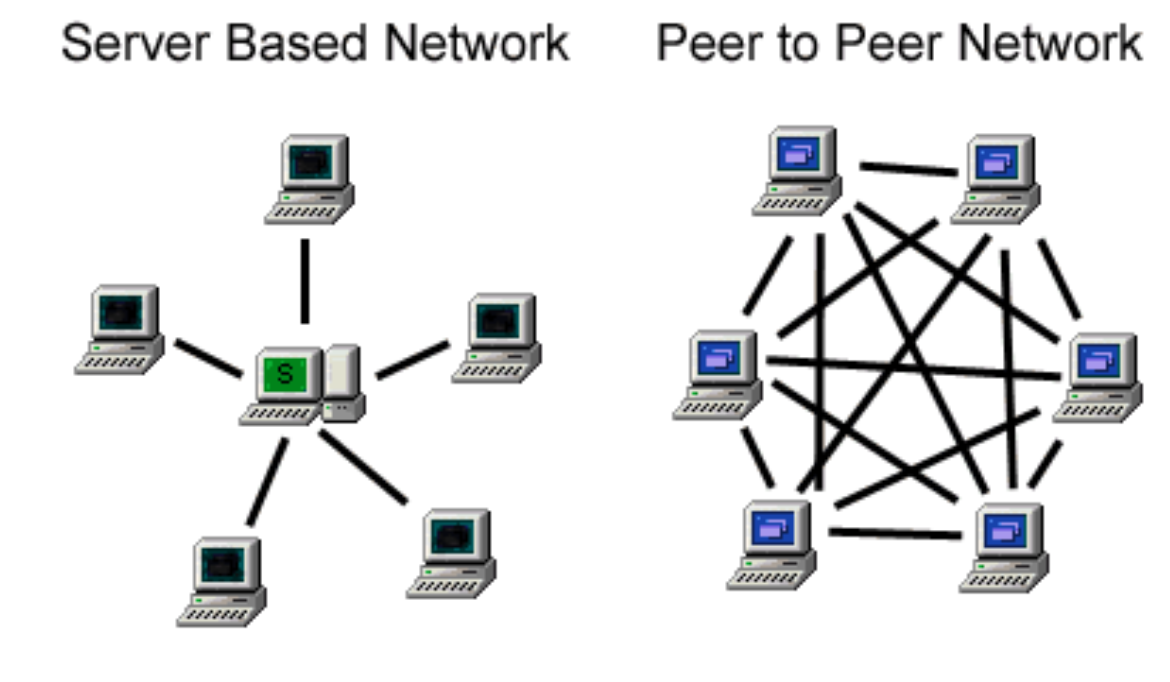
\includegraphics[width=0.7\textwidth]{blockchain.png}
    \caption{An example of a blockchain structure.}
    \label{fig:blockchain_structure}
\end{figure}

\subsection{Types of Blockchains}
Blockchains can be categorized into several types based on their access control and consensus mechanisms:
\begin{itemize}
    \item \textbf{Public Blockchains}: Open to anyone, allowing anyone to participate in the network (e.g., Bitcoin, Ethereum).
    \item \textbf{Private Blockchains}: Restricted access, typically used by organizations for internal purposes (e.g., Hyperledger Fabric).
    \item \textbf{Consortium Blockchains}: Controlled by a group of organizations, combining elements of public and private blockchains (e.g., R3 Corda).
    \item \textbf{Hybrid Blockchains}: Combine features of both public and private blockchains, allowing for selective transparency (e.g., Dragonchain).
\end{itemize}
\subsection{Ledger \& Nodes}
A ledger is a digital record-keeping system that maintains a chronological list of transactions or data entries. In blockchain, the ledger is distributed across a network of nodes, ensuring transparency and security. Each node stores a copy of the entire ledger, allowing for decentralized validation and consensus. This structure prevents tampering, as altering any entry would require changing it across all nodes simultaneously. The ledger's immutability and transparency are fundamental to blockchain's trustless nature, enabling secure peer-to-peer transactions without intermediaries.
\subsection{Blocks}
Blocks are the fundamental units of a blockchain, containing a collection of transactions or data entries. Each block consists of a header (which includes metadata like the previous block's hash, timestamp, and nonce) and a body (which contains the actual transaction data). Blocks are linked together in chronological order, forming an immutable chain. When a new block is added, it references the hash of the previous block, ensuring continuity and security. This structure prevents tampering, as altering any block would require recalculating all subsequent blocks' hashes. Blocks are validated through consensus mechanisms like Proof of Work or Proof of Stake, ensuring that only legitimate transactions are recorded on the blockchain.
\subsection{Transactions}
Transactions are the core operations in a blockchain, representing the transfer of assets or data between participants. Each transaction is digitally signed by the sender using their private key, ensuring authenticity and integrity. Once initiated, transactions are broadcast to the network, where nodes validate them against consensus rules (e.g., checking for sufficient funds, verifying signatures). Validated transactions are grouped into blocks and added to the blockchain in a sequential manner. This process creates a transparent, tamper-proof record of all transactions, enabling trustless interactions without intermediaries. Transactions can involve various assets, such as cryptocurrencies, tokens, or smart contract executions, depending on the blockchain's functionality.



\section{Cryptographic Fundamentals}
Cryptography is the backbone of blockchain security, ensuring data integrity, confidentiality, and authenticity.Cryptography secures blockchain by ensuring tamper-proof data and trustless transactions. It uses hash functions (like SHA-256) to link blocks immutably, public-key encryption for secure identities and signatures, and Merkle trees for efficient transaction verification. These techniques create a decentralized system where no central authority is needed—math alone guarantees security and integrity.
\subsection{What is hashing?}
Hashing is a cryptographic process that converts input data (like transactions) into a fixed-length alphanumeric string called a hash, unique to each input. Even a tiny change in input creates a completely different hash, making tampering evident. Blockchain uses hashing (e.g., SHA-256 in Bitcoin) to link blocks securely—each block contains the hash of the previous block, forming an immutable chain. Hashes also enable efficient data verification without exposing original data, ensuring both integrity and privacy. This one-way function is fundamental to blockchain’s security and structure.

\subsection{Hash Functions/Algorithms}
Hash functions are cryptographic algorithms that transform input data of any size into a fixed-length, unique alphanumeric string called a hash. These deterministic yet irreversible functions ensure data integrity—even a minor change in input (like a single character) produces a completely different output (avalanche effect). Blockchains rely on secure hash algorithms like SHA-256 (Bitcoin) and Keccak-256 (Ethereum) to link blocks immutably: each block’s header includes the hash of the previous block, creating a tamper-evident chain. The computational infeasibility of reverse-engineering or finding two inputs with the same hash (collision resistance) makes them vital for verifying transactions, securing digital signatures, and maintaining consensus. By converting arbitrary data into compact, unforgeable fingerprints, hash functions enable blockchain’s trustless transparency without compromising efficiency.
\begin{figure}[h]
    \centering
    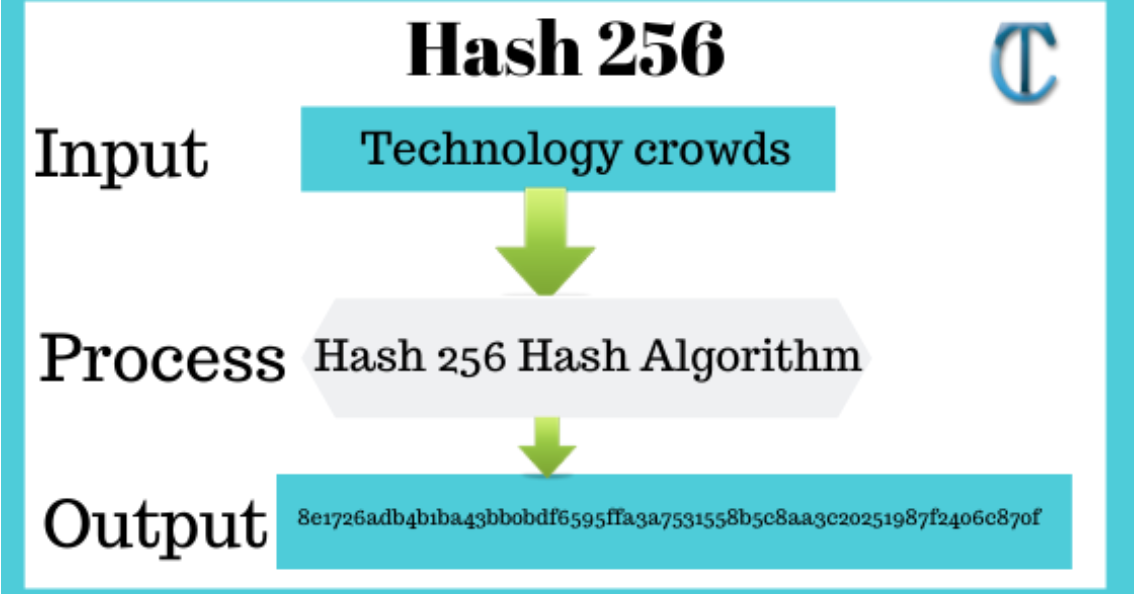
\includegraphics[width=0.7\textwidth]{Compute-Hash-256.png}
    \caption{An example of a hashing process.}
    \label{fig:hashing_example}
\end{figure}
\subsection{Public Key and private key}
In blockchain, public and private keys form the foundation of secure transactions and digital identities. A private key (a randomly generated 256-bit number) acts as a secret password to authorize transactions and access funds. Its paired public key is derived mathematically from the private key and serves as an address to receive funds. While the public key is shareable, the private key must remain confidential—anyone with it can control associated assets. Transactions are signed with the private key and verified by others using the public key, ensuring authenticity without revealing sensitive information. This asymmetric cryptography enables trustless interactions, as users can prove ownership without exposing credentials. Losing a private key means permanent loss of access, while compromised keys risk theft. Together, they secure wallets, enable smart contracts, and power blockchain’s permissionless trust model.
\subsection{Digital Signatures}
Digital signatures provide a secure way to verify the authenticity and integrity of data in blockchain transactions. When a user (Person A) signs a document or transaction, they use their private key to generate a unique cryptographic signature. This signature, along with the original data's hash, can only be decoded and validated using the corresponding public key, proving the data originated from Person A and hasn’t been altered. The process ensures non-repudiation—since only the private key holder could have created the signature—and tamper-proofing, as any change to the data would invalidate the hash. Anyone on the network can verify the signature using the signer’s public key, enabling trustless validation without revealing the private key. This mechanism underpins secure transactions, smart contracts, and identity verification in blockchain systems, combining transparency with robust security.
\section{BitCoin}
\subsection{Origin of Bitcoin}
Bitcoin emerged in 2008 when the pseudonymous Satoshi Nakamoto published its whitepaper, launching the first decentralized cryptocurrency in 2009. Designed as open-source software, Bitcoin introduced a peer-to-peer electronic cash system with a predetermined maximum supply of 21 million coins, creating digital scarcity analogous to precious metals. This innovation solved the double-spending problem without requiring trusted third parties.
\begin{figure}[h]
    \centering
    
\includegraphics[width=0.7\textwidth]{bitcoin.png}
    \caption{Bitcoin}
    \label{Bitcoin}
\end{figure}
\subsection{Bitcoin's Operational Framework}
Bitcoin operates on a decentralized, peer-to-peer network where transactions are verified by nodes through cryptographic proof. It uses a Proof-of-Work consensus mechanism, requiring miners to solve complex mathematical puzzles to add new blocks to the blockchain. Each block contains a list of transactions, a timestamp, and the hash of the previous block, ensuring immutability. Bitcoin's supply is capped at 21 million coins, with new bitcoins created through mining rewards that halve approximately every four years (the "halving" event). This deflationary model aims to mimic scarce resources like gold, promoting long-term value retention. Transactions are pseudonymous, recorded on a public ledger accessible to anyone, enhancing transparency while preserving user privacy.
\subsection{Collaborative Mining Approach}
Mining pools represent a collective solution to increasing mining difficulty:
Multiple miners combine computational resources to improve block discovery probabilityRewards are distributed proportionally based on contributed hash powerEnables consistent returns for individual miners despite rising competitionThis model preserves network decentralization while addressing economic viability concerns.
\subsection{Elliptic Curve Digital Signature Algorithm (ECDSA)}
ECDSA (Elliptic Curve Digital Signature Algorithm) is a way to make sure messages are real and safe. It uses special math called elliptic curve cryptography. ECDSA makes a secret key that only the sender knows and a public key that everyone can see. The secret key is used to sign the message. The public key is used to check if the signature is real. This helps to stop people from changing the message or pretending to be someone else. People use ECDSA in many places, like Bitcoin, secure websites, and secure messages. It’s strong and safe, even when the keys are small, so it works quickly. That’s why ECDSA is popular for keeping messages safe and making sure they are real.
\subsection{UTXOs}
Bitcoin transactions use a system known as Unspent Transaction Outputs (UTXOs). In
essence, UTXOs define where each blockchain transaction starts and finishes. What this
does is each transaction uses one or more UTXOs as inputs and generates new UTXOs
as outputs. This structure ensures the traceability of all Bitcoin transactions.
\section{Ethereum}
\subsection{Evolution of Ethereum}
Ethereum emerged in 2015 as a revolutionary evolution beyond Bitcoin's digital cash system. While Bitcoin was designed primarily as decentralized money, Ethereum introduced smart contracts—self-executing code that enables complex applications to run on its blockchain. The key difference lies in functionality: Bitcoin is a payment network, whereas Ethereum is a programmable platform for building decentralized applications (dApps), tokens (like ERC-20), and decentralized organizations (DAOs). Ethereum's native cryptocurrency, Ether (ETH), fuels transactions and computational services on the network. Its flexibility supports use cases like DeFi, NFTs, and Web3, making it a foundational technology for the decentralized internet. Unlike Bitcoin's fixed monetary policy, Ethereum continuously evolves through upgrades (e.g., PoS transition) to improve scalability and sustainability.
\begin{figure}[h]
    \centering
    
\includegraphics[width=0.7\textwidth]{ethereum.png}
    \caption{ethereum}
    \label{fig:ethereum_example}
\end{figure}
\subsection{Ether}
Ether (ETH) is the native cryptocurrency of the Ethereum blockchain, serving as both a digital currency and a utility token. It powers transactions, smart contracts, and decentralized applications (dApps) on the Ethereum network. Ether is used to pay for computational services (gas fees) required to execute operations on the blockchain, incentivizing miners or validators to maintain network security. Unlike Bitcoin's fixed supply, Ether's issuance is dynamic, with new ETH created through mining or staking rewards. This flexibility supports Ethereum's evolving ecosystem, enabling developers to build diverse applications ranging from decentralized finance (DeFi) platforms to non-fungible tokens (NFTs). As a versatile asset, Ether plays a crucial role in driving innovation within the blockchain space.
\subsection{Smart Contracts}
Smart contracts are self-executing agreements with terms written directly into code, deployed on blockchains like Ethereum. These contracts automatically execute when predefined conditions are met, eliminating intermediaries. For example, a smart contract could release payment automatically upon delivery confirmation. By running on decentralized networks, they ensure tamper-proof, transparent, and trustless transactions, powering applications like DeFi protocols, NFT marketplaces, and supply chain automation. Their immutability and autonomy make them fundamental to blockchain's disruptive potential.
\subsection{Ethereum's Operational Framework}
Ethereum operates as a decentralized platform enabling developers to build and deploy smart contracts and dApps. It uses a Proof-of-Stake (PoS) consensus mechanism, transitioning from Proof-of-Work (PoW) to enhance scalability and energy efficiency. Ethereum's blockchain consists of blocks containing transaction data, smart contract code, and state changes. The Ethereum Virtual Machine (EVM) executes smart contracts, allowing for complex logic and interactions. Ether (ETH) serves as the native cryptocurrency, used for transaction fees (gas) and staking in the PoS system. This architecture supports a wide range of applications, from decentralized finance (DeFi) to non-fungible tokens (NFTs), fostering innovation in the blockchain ecosystem.
\subsection{Etherium virtual machine}
The Ethereum Virtual Machine (EVM) is a decentralized, Turing-complete runtime environment that executes smart contracts on the Ethereum blockchain. It serves as a global computer, allowing developers to deploy and run code in a secure, trustless manner. The EVM processes transactions, manages state changes, and enforces consensus across the network. Each node in the Ethereum network runs an instance of the EVM, ensuring consistent execution of smart contracts. This enables complex applications like decentralized finance (DeFi), non-fungible tokens (NFTs), and decentralized autonomous organizations (DAOs) to operate seamlessly on the blockchain. The EVM's design promotes interoperability and innovation within the Ethereum ecosystem.
\subsection{Ethereum Wallets \& Transactions}
Ethereum wallets are tools that store your Ether (ETH) and let you do things like sending and receiving money. Each wallet has a public address, which you can share with people to receive ETH, and a private key, which is like your secret password—never share it with anyone! There are different types of wallets: some are software apps like MetaMask, while others are physical devices (hardware wallets). When you want to send ETH or interact with smart contracts, you have to pay a fee called “gas.” This fee goes to the people (validators) who help run the network. Using a wallet is one of the first things you’ll do with Ethereum, so it’s important to learn how to create one and practice making small transactions on a test network.
\subsection{Test Networks}
Test networks, or testnets, are blockchain environments that simulate the main network (mainnet) for testing purposes. They allow developers to deploy and test smart contracts, dApps, and other functionalities without risking real assets. Testnets use their own native tokens (e.g., Ropsten, Rinkeby, Goerli for Ethereum) that hold no real value, enabling experimentation with zero financial risk. These networks help identify bugs, optimize code, and ensure security before deploying on the mainnet. Testnets are essential for fostering innovation in blockchain development while maintaining the integrity of the main network.
\subsection{Mining}
Ethereum originally used Proof-of-Work (PoW) mining, where miners competed to solve cryptographic puzzles using GPUs to validate transactions and create new blocks. Successful miners earned block rewards (ETH) and transaction fees. Unlike Bitcoin's ASIC-dominated mining, Ethereum's Ethash algorithm favored GPU rigs, making mining more accessible. However, rising energy costs and centralization concerns led to Ethereum's transition to Proof-of-Stake (PoS) in 2022 ("The Merge"), permanently replacing miners with validators who stake ETH. Pre-Merge mining laid Ethereum's foundation but was phased out for sustainability.
\subsection{Staking}
Staking is the process of locking up Ether (ETH) to participate in Ethereum's Proof-of-Stake (PoS) consensus and earn rewards. Validators stake a minimum of 32 ETH to verify transactions and propose blocks, or users can join staking pools with smaller amounts. Unlike energy-intensive mining, staking secures the network efficiently while yielding 4-6 \% annual returns (variable). Stakers help maintain Ethereum's security and decentralization, but face slashing risks for malicious behavior. Post-Merge, staking replaced mining as Ethereum's validation mechanism.
\subsection{Gas fees}
Gas fees are transaction costs on the Ethereum network, paid in Ether (ETH) to compensate validators for processing and validating transactions. Each operation in a smart contract or transaction consumes a certain amount of gas, which is priced based on network demand. Users specify a gas limit (maximum amount they are willing to pay) and a gas price (amount per unit of gas). When the network is congested, gas prices rise, incentivizing validators to prioritize transactions with higher fees. Gas fees ensure fair resource allocation, prevent spam attacks, and maintain network security. They vary dynamically based on network activity, making them a crucial aspect of Ethereum's economic model.
\subsection{Deccentralized applications (Dapps)}
dApps are applications that run on a decentralized network, such as Ethereum. They use smart contracts for their backend logic, providing increased security, transparency,and resistance to censorship. Examples of dApps include decentralized finance (DeFi)platforms, gaming applications, and supply chain management tools.
\subsection{ICO vs. IPO: Key Differences}
An Initial Coin Offering (ICO) is a blockchain-based fundraising method where startups sell newly created tokens to investors, similar to how an Initial Public Offering (IPO) offers company shares to the public. While IPOs are heavily regulated and require compliance with securities laws, ICOs operate with minimal oversight, making them faster but riskier. ICOs are popular among crypto projects to raise capital for decentralized platforms, whereas IPOs represent traditional equity ownership in companies. The lack of regulation in ICOs can lead to scams or failed projects, whereas IPOs provide investor protections but with stricter entry barriers. Both aim to secure funding, but ICOs offer tokens (often utility-based), while IPOs issue shares (ownership stakes).
\subsection{Sharding}
Sharding is a scalability technique used in blockchain networks to increase transaction throughput and reduce latency. In traditional blockchains, every node processes and stores the entire transaction history, which can lead to bottlenecks as the network grows. Sharding addresses this by dividing the blockchain into smaller, manageable segments called "shards." Each shard processes its own subset of transactions and smart contracts independently, allowing multiple transactions to be handled in parallel. In Ethereum, sharding is a key component of planned upgrades to improve scalability. Validators are assigned to specific shards, and cross-shard communication protocols ensure data consistency and security across the network. By distributing the workload, sharding enables blockchains to support more users and applications without sacrificing decentralization or security. However, implementing sharding introduces new challenges, such as ensuring secure cross-shard transactions and preventing certain types of attacks, which are active areas of research and development.
\subsection{Real-Life Uses of Ethereum}
\begin{itemize}
    \item \textbf{Decentralized Finance (DeFi)}: Platforms like Uniswap and Aave enable peer-to-peer lending, borrowing, and trading without intermediaries.
    \item \textbf{Non-Fungible Tokens (NFTs)}: Ethereum powers NFT marketplaces like OpenSea, allowing artists to tokenize and sell digital art.
    \item \textbf{Decentralized Autonomous Organizations (DAOs)}: Organizations like MakerDAO use smart contracts for governance and decision-making without central authority.
    \item \textbf{Supply Chain Management}: Companies like VeChain use Ethereum to track products through transparent, tamper-proof ledgers.
    \item \textbf{Gaming and Virtual Worlds}: Games like Axie Infinity leverage Ethereum for in-game assets and economies, enabling true ownership of digital items.
    \item \textbf{Identity Verification}: Projects like uPort use Ethereum to create self-sovereign identities, allowing users to control their personal data.
    \item \textbf{Crowdfunding and Token Sales}: Ethereum facilitates Initial Coin Offerings (ICOs) and token sales, enabling startups to raise capital directly from the community.    
\end{itemize}
\section{Smart Contracts}
Smart contracts are self-executing programs stored on a blockchain that automatically run when predefined conditions are met. They remove the need for intermediaries by enforcing trust through code, enabling secure and decentralized applications (DApps) like payments, voting, and asset sharing. To write and deploy these contracts on the Ethereum blockchain, developers use Solidity, a high-level programming language specifically designed for smart contract development. Solidity lets you define contract logic, data storage, and rules for how users interact with the blockchain. However, a smart contract alone is not enough — users need a way to interact with it. This is where the frontend comes in. A frontend is a web-based interface built using tools like React, Vite, and Tailwind CSS, which communicates with the smart contract using ethers.js or web3.js. To run the frontend locally, basic requirements include Node.js, npm, MetaMask (to connect to Ethereum wallets), and libraries like ethers for blockchain communication. With a clean and interactive UI, users can connect their wallets, perform transactions, view balances, and settle expenses — all powered by the underlying smart contract on the blockchain.
\subsection{Solidity}
\subsubsection{What is Solidity?}
Solidity is an object-oriented, high-level language for implementing smart contracts. Smart contracts are programs that govern the behavior of accounts within the Ethereum state. Solidity is a curly-bracket language designed to target the Ethereum Virtual Machine (EVM). It is influenced by C++, Python, and JavaScript. You can find more details about which languages Solidity has been inspired by in the language influences section. Solidity is statically typed, supports inheritance, libraries, and complex user-defined types, among other features. With Solidity, you can create contracts for uses such as voting, crowdfunding, blind auctions, and multi-signature wallets. When deploying contracts, you should use the latest released version of Solidity. Apart from exceptional cases, only the latest version receives security fixes. Furthermore, breaking changes, as well as new features, are introduced regularly. We currently use a 0.y.z version number to indicate this fast pace of change.
\subsubsection{Sample code in solidity}
\begin{verbatim}
    // SPDX-License-Identifier: GPL-3.0
    pragma solidity >=0.4.16 <0.9.0;

    contract SimpleStorage {
        uint storedData;

        function set(uint x) public {
            storedData = x;
        }

        function get() public view returns (uint) {
            return storedData;
        }
    }
\end{verbatim}
\begin{itemize}
    \item The first line tells you that the source code is licensed under the GPL version 3.0. Machine-readable license specifiers are important in a setting where publishing the source code is the default.
    \item The next line specifies that the source code is written for Solidity version 0.4.16, or a newer version of the language up to, but not including version 0.9.0. This is to ensure that the contract is not compilable with a new (breaking) compiler version, where it could behave differently. Pragmas are common instructions for compilers about how to treat the source code (e.g. pragma once).
    \item To access a member (like a state variable) of the current contract, you do not typically add the this. prefix, you just access it directly via its name. Unlike in some other languages, omitting it is not just a matter of style, it results in a completely different way to access the member, but more on this later.
    \item This contract does not do much yet apart from (due to the infrastructure built by Ethereum) allowing anyone to store a single number that is accessible by anyone in the world without a (feasible) way to prevent you from publishing this number. Anyone could call set again with a different value and overwrite your number, but the number is still stored in the history of the blockchain. Later, you will see how you can impose access restrictions so that only you can alter the number.
\end{itemize}
\subsubsection{File Structure}
Every Solidity file begins with a license identifier and a compiler version.
\begin{verbatim}
    // SPDX-License-Identifier: MIT
    pragma solidity ^0.8.0;
\end{verbatim}
\subsubsection{Basics of Solidity}
\textbf{Data Types:}
\textbf{Value Types:}
\begin{itemize}
    \item \textbf{Boolean}: Represents true or false values.
    \item \textbf{Integer}: Signed and unsigned integers of various sizes (e.g., int8, uint256).
    \item \textbf{Address}: Holds Ethereum addresses.
    \item \textbf{Fixed Point Numbers}: Not supported natively, but can be implemented using libraries.
\end{itemize}
\textbf{Reference Types:}
\begin{itemize}
    \item \textbf{Arrays}: Fixed-size or dynamic arrays of value types or other reference types.
    \item \textbf{Structs}: Custom data structures that group related data together.
    \item \textbf{Mappings}: Key-value pairs that allow efficient data retrieval.
\end{itemize}
\textbf{Variables in Solidity}
\begin{itemize}
    \item \textbf{State Variables}: Variables that are permanently stored in the contract's storage.
    \begin{verbatim}
        uint256 public myNumber;
    \end{verbatim}
    \item \textbf{Local Variables}: Variables that are declared inside a function and only exist during its execution.
    \begin{verbatim}
        function myFunction() public {
            uint256 localVar = 5;
        }
    \end{verbatim}
    \item \textbf{Global Variables}: Built-in variables that provide information about the blockchain or the contract's environment.
    \begin{verbatim}
        address public owner = msg.sender; // The address of the contract creator
        uint256 public blockNumber = block.number; // Current block number
    \end{verbatim}
    \item \textbf{Constants}: Immutable variables that cannot be changed after declaration.
    \begin{verbatim}
        uint256 public constant MAX_VALUE = 1000; // A constant value
    \end{verbatim}
\end{itemize}
\subsubsection{Functions in Solidity}
\textbf{Function Declaration:}
Functions are declared with the `function` keyword, followed by a name, parameters (if any), and a return type (if applicable).
\begin{verbatim}
    function myFunction(uint256 param) public returns (uint256) {
        return param * 2;
    }
\end{verbatim}
\textbf{Function Modifiers:}
Modifiers are used to change the behavior of functions. Common modifiers include `view`, `pure`, and `payable`.
\begin{verbatim}
    function myViewFunction() public view returns (uint256) {
        return myNumber;
    }
\end{verbatim}
\textbf{Example:}
Here’s a simple contract with a function that increments a number:
\begin{verbatim}
    pragma solidity ^0.8.0;

    contract Incrementer {
        uint256 public myNumber;

        function increment() public {
            myNumber++;
        }
    }
\end{verbatim}
\subsubsection{Function visibility}
Function visibility determines which contracts and functions can call a particular function. There are four visibility specifiers: public, external, internal, and private. They control how accessible a function is, both within and outside the defining contract. It is like access specifiers in other OOP languages such as C++.
\textbf{Public:} Functions declared as public can be called from anywhere, both internally and externally. They are accessible to other contracts and transactions.
\begin{verbatim}
    function myPublicFunction() public {
        // Function logic here
    }
\end{verbatim}
\textbf{External:} External functions can only be called from outside the contract. They are not accessible internally, meaning they cannot be called by other functions within the same contract.
\begin{verbatim}
    function myExternalFunction() external {
        // Function logic here
    }
\end{verbatim}
\textbf{Internal:} Internal functions can only be called from within the contract itself or from derived contracts. They are not accessible externally.
\begin{verbatim}
    function myInternalFunction() internal {
        // Function logic here
    }
\end{verbatim}
\textbf{Private:} Private functions can only be called from within the contract itself. They are not accessible to derived contracts or external calls.
\begin{verbatim}
    function myPrivateFunction() private {
        // Function logic here
    }
\end{verbatim}
\textbf{Example:}
Here’s a simple contract demonstrating different visibility levels:
\begin{verbatim}
    pragma solidity ^0.8.0;

    contract VisibilityExample {
        uint256 private secretNumber;
        uint256 public publicNumber;

        function setSecretNumber(uint256 _num) private {
            secretNumber = _num;
        }

        function setPublicNumber(uint256 _num) public {
            publicNumber = _num;
        }

        function getSecretNumber() internal view returns (uint256) {
            return secretNumber;
        }

        function getPublicNumber() external view returns (uint256) {
            return publicNumber;
        }
    }
\end{verbatim}
\subsubsection{Constructors}
A constructor is a special function that runs only once — when the contract is deployed. It is used to initialize contract variables or perform setup steps like assigning the owner. Runs automatically when the contract is deployed. Cannot be called again after deployment. Usually used to set the owner, initial values, etc.
\begin{verbatim}
    contract MyContract {
        address public owner;

        constructor() {
            owner = msg.sender; // Set the contract creator as the owner
        }
    }
\end{verbatim}
In this example, the `constructor` sets the `owner` variable to the address of the contract creator (`msg.sender`). This ensures that the contract has an owner from the moment it is deployed
\subsubsection{Modifiers}
Modifiers are used to change the behavior of functions. They can be used to add preconditions, postconditions, or to modify the input/output of functions. Here’s an example of a simple modifier:
\begin{verbatim}
    modifier onlyOwner() {
        require(msg.sender == owner, "Not the contract owner");
        _;
    }
\end{verbatim}
In this example, the `onlyOwner` modifier checks if the caller is the contract owner. If the condition is met, the function execution continues; otherwise, it reverts with an error message. Modifiers can be applied to functions like this:
\begin{verbatim}
    function restrictedFunction() public onlyOwner {
        // Function logic here
    }
\end{verbatim}
\subsubsection{Events}
Events are used to log information on the blockchain, allowing external applications to listen for specific occurrences in
the contract. They are useful for tracking state changes or important actions. Here’s an example of how to define and emit an event:
\begin{verbatim}
    event NumberUpdated(uint256 newNumber);
\end{verbatim}
In this example, the `NumberUpdated` event is defined to log when a number is updated. To emit this event, you can use the `emit` keyword within a function:
\begin{verbatim}
    function updateNumber(uint256 _newNumber) public {
        myNumber = _newNumber;
        emit NumberUpdated(_newNumber);
    }
\end{verbatim}
In this example, when the `updateNumber` function is called, it updates the `myNumber` variable and emits the `NumberUpdated` event with the new value. External applications can listen for this event to track changes in the contract's state.
\subsubsection{Storage and Memory}
In Solidity, data can be stored in two main locations: storage and memory. Understanding the differences between these two is crucial for efficient contract development.
\textbf{Storage:} Storage is where all state variables are permanently stored on the blockchain. It is persistent and retains data between function calls and transactions. Modifying storage variables incurs gas costs, as it requires writing to the blockchain.
\begin{verbatim}
    contract StorageExample {
        uint256 public storedData; // Stored in blockchain storage
        function setStoredData(uint256 _data) public {
            storedData = _data;
        }
    }
\end{verbatim}
\textbf{Memory:} Memory is a temporary storage area used for variables that only exist during the execution of a function. It is not persistent and does not incur gas costs for storage operations. Memory is typically used for function parameters and local variables.
\begin{verbatim}
    contract MemoryExample {
        function calculateSum(uint256 a, uint256 b) public pure returns (uint256) {
            uint256 sum = a + b; // Stored in memory
            return sum;
        }
    }
\end{verbatim}
\textbf{Example:}
Here’s a simple contract demonstrating the use of storage and memory:
\begin{verbatim}
    pragma solidity ^0.8.0;

    contract StorageMemoryExample {
        uint256 public storedData; // Stored in blockchain storage

        function setStoredData(uint256 _data) public {
            storedData = _data;
        }

        function getStoredData() public view returns (uint256) {
            return storedData;
        }

        function calculateSum(uint256 a, uint256 b) public pure returns (uint256) {
            uint256 sum = a + b; // Stored in memory
            return sum;
        }
    }
\end{verbatim}
\subsubsection{Inheritance}
Inheritance in Solidity allows contracts to inherit properties and behaviors from other contracts, promoting code reuse and modularity. It enables developers to create a hierarchy of contracts, where child contracts can extend or override the functionality of parent contracts. This is similar to inheritance in object-oriented programming languages like C++ or Java
\begin{verbatim}
    contract ParentContract {
        uint256 public parentData;

        function setParentData(uint256 _data) public {
            parentData = _data;
        }
    }

    contract ChildContract is ParentContract {
        uint256 public childData;

        function setChildData(uint256 _data) public {
            childData = _data;
        }
    }
\end{verbatim}
In this example, `ChildContract` inherits from `ParentContract`, allowing it to access the `parentData` variable and the `setParentData` function. The child contract can also define its own variables and functions, such as `childData` and `setChildData`. This inheritance allows for a clear separation of concerns and promotes code reuse, making it easier to maintain and extend contracts
\subsubsection{Interfaces}
Interfaces in Solidity define a contract's external functions without implementing them, allowing other contracts to interact with them. They serve as a blueprint for contracts, specifying the functions that must be implemented by any contract that inherits from the interface. This promotes modularity and interoperability between contracts, enabling developers to create flexible and reusable code.
\begin{verbatim}
    interface IExample {
        function getValue() external view returns (uint256);
        function setValue(uint256 _value) external;
    }   
\end{verbatim}
In this example, `IExample` is an interface that defines two external functions: `getValue` and `setValue`. Any contract that implements this interface must provide concrete implementations for these functions. This allows other contracts to interact with `IExample` without needing to know the specific implementation details
\begin{verbatim}
    contract ExampleContract is IExample {
        uint256 private value;

        function getValue() external view override returns (uint256) {
            return value;
        }

        function setValue(uint256 _value) external override {
            value = _value;
        }
    }
\end{verbatim}
\section{Gas optimization}
Every operation on the Ethereum blockchain costs gas, which is paid in ETH. The more complex your contract is, or the more data it stores and processes, the more expensive it becomes. That’s why it’s important to write smart contracts that are optimized to use less gas. Gas optimization means writing code in a way that uses less storage, fewer computations, and simpler logic, without changing what your contract does. This makes the contract cheaper to use and faster to run.
\begin{itemize}
    \item \textbf{Use Smaller Data Types:} Use the smallest data type that fits your needs. For example, if you only need numbers between 0 and 255, use `uint8` instead of `uint256`.
    \item \textbf{Avoid Unnecessary Storage:} Minimize the use of storage variables, as they are more expensive than memory variables. Use memory for temporary data that doesn’t need to be stored permanently.
    \item \textbf{Batch Operations:} Instead of performing multiple operations in separate transactions, batch them into a single transaction to save on gas costs.
    \item \textbf{Use Libraries:} Libraries can help reduce code duplication and save gas. Use libraries for common functions that can be reused across contracts.
    \item \textbf{Optimize Loops:} Avoid loops that iterate over large arrays or mappings. If necessary, limit the number of iterations or use more efficient data structures.
    \item \textbf{Avoid Dynamic Arrays:} Dynamic arrays can be more expensive than fixed-size arrays. If possible, use fixed-size arrays to save on gas costs.
    \item \textbf{Use Events Wisely:} Emit events only when necessary, as they consume gas. Use them to log important state changes or actions, but avoid excessive logging.
    \item \textbf{Minimize Function Calls:} Each function call incurs gas costs. Minimize the number of function calls, especially in loops or frequently called functions.
    \item \textbf{Use View and Pure Functions:} Use `view` and `pure` functions whenever possible, as they do not modify the state and are cheaper to call. They can be used for read-only operations or calculations that do not require state changes.
    \item \textbf{Avoid Redundant Calculations:} Store results of expensive calculations in state variables instead of recalculating them multiple times. This reduces gas costs for repeated operations.
    \item \textbf{Use Short-Circuiting Logic:} Use short-circuiting logic in conditional statements to avoid unnecessary evaluations. For example, use `\&\&` (AND) and `||` (OR) operators to skip evaluations when the result is already determined.
    \item \textbf{Optimize Contract Size:} Keep your contract size small to avoid hitting the maximum bytecode size limit. This can be achieved by removing unnecessary functions, comments, and whitespace.
    \item \textbf{Use Fixed-Size Arrays:} Fixed-size arrays are cheaper than dynamic arrays. If you know the size of the array in advance, use fixed-size arrays to save on gas costs.
    \item \textbf{Avoid Unused Variables:} Remove any unused variables or functions from your contract. They consume gas during deployment and execution, even if they are not used.
    \item \textbf{Use Efficient Data Structures:} Choose data structures that are efficient for your use case. For example, use mappings for key-value pairs instead of arrays for lookups, as mappings provide constant time complexity for access.
    \item \textbf{Minimize External Calls:} External calls to other contracts can be expensive. Minimize the number of external calls and ensure they are necessary for your contract's functionality.
    \item \textbf{Use Inline Assembly:} For advanced users, inline assembly can be used to optimize specific operations. However, this should be done with caution, as it can make the code harder to read and maintain.
    \item \textbf{Profile and Test:} Use tools like Remix, Hardhat, or Truffle to profile your contract's gas usage. Regularly test and optimize your contract to identify areas where gas consumption can be reduced.
    \item \textbf{Stay Informed:} Keep up with the latest developments in Ethereum and Solidity. New optimizations and best practices are constantly being discovered, so staying informed can help you write more efficient contracts.
\end{itemize}
\section{Deploying Smart Contracts}
\subsection{Write the Solidity Code}
Use Remix IDE and write the smart contract in a .sol file.
\begin{figure}[h]
    \centering
    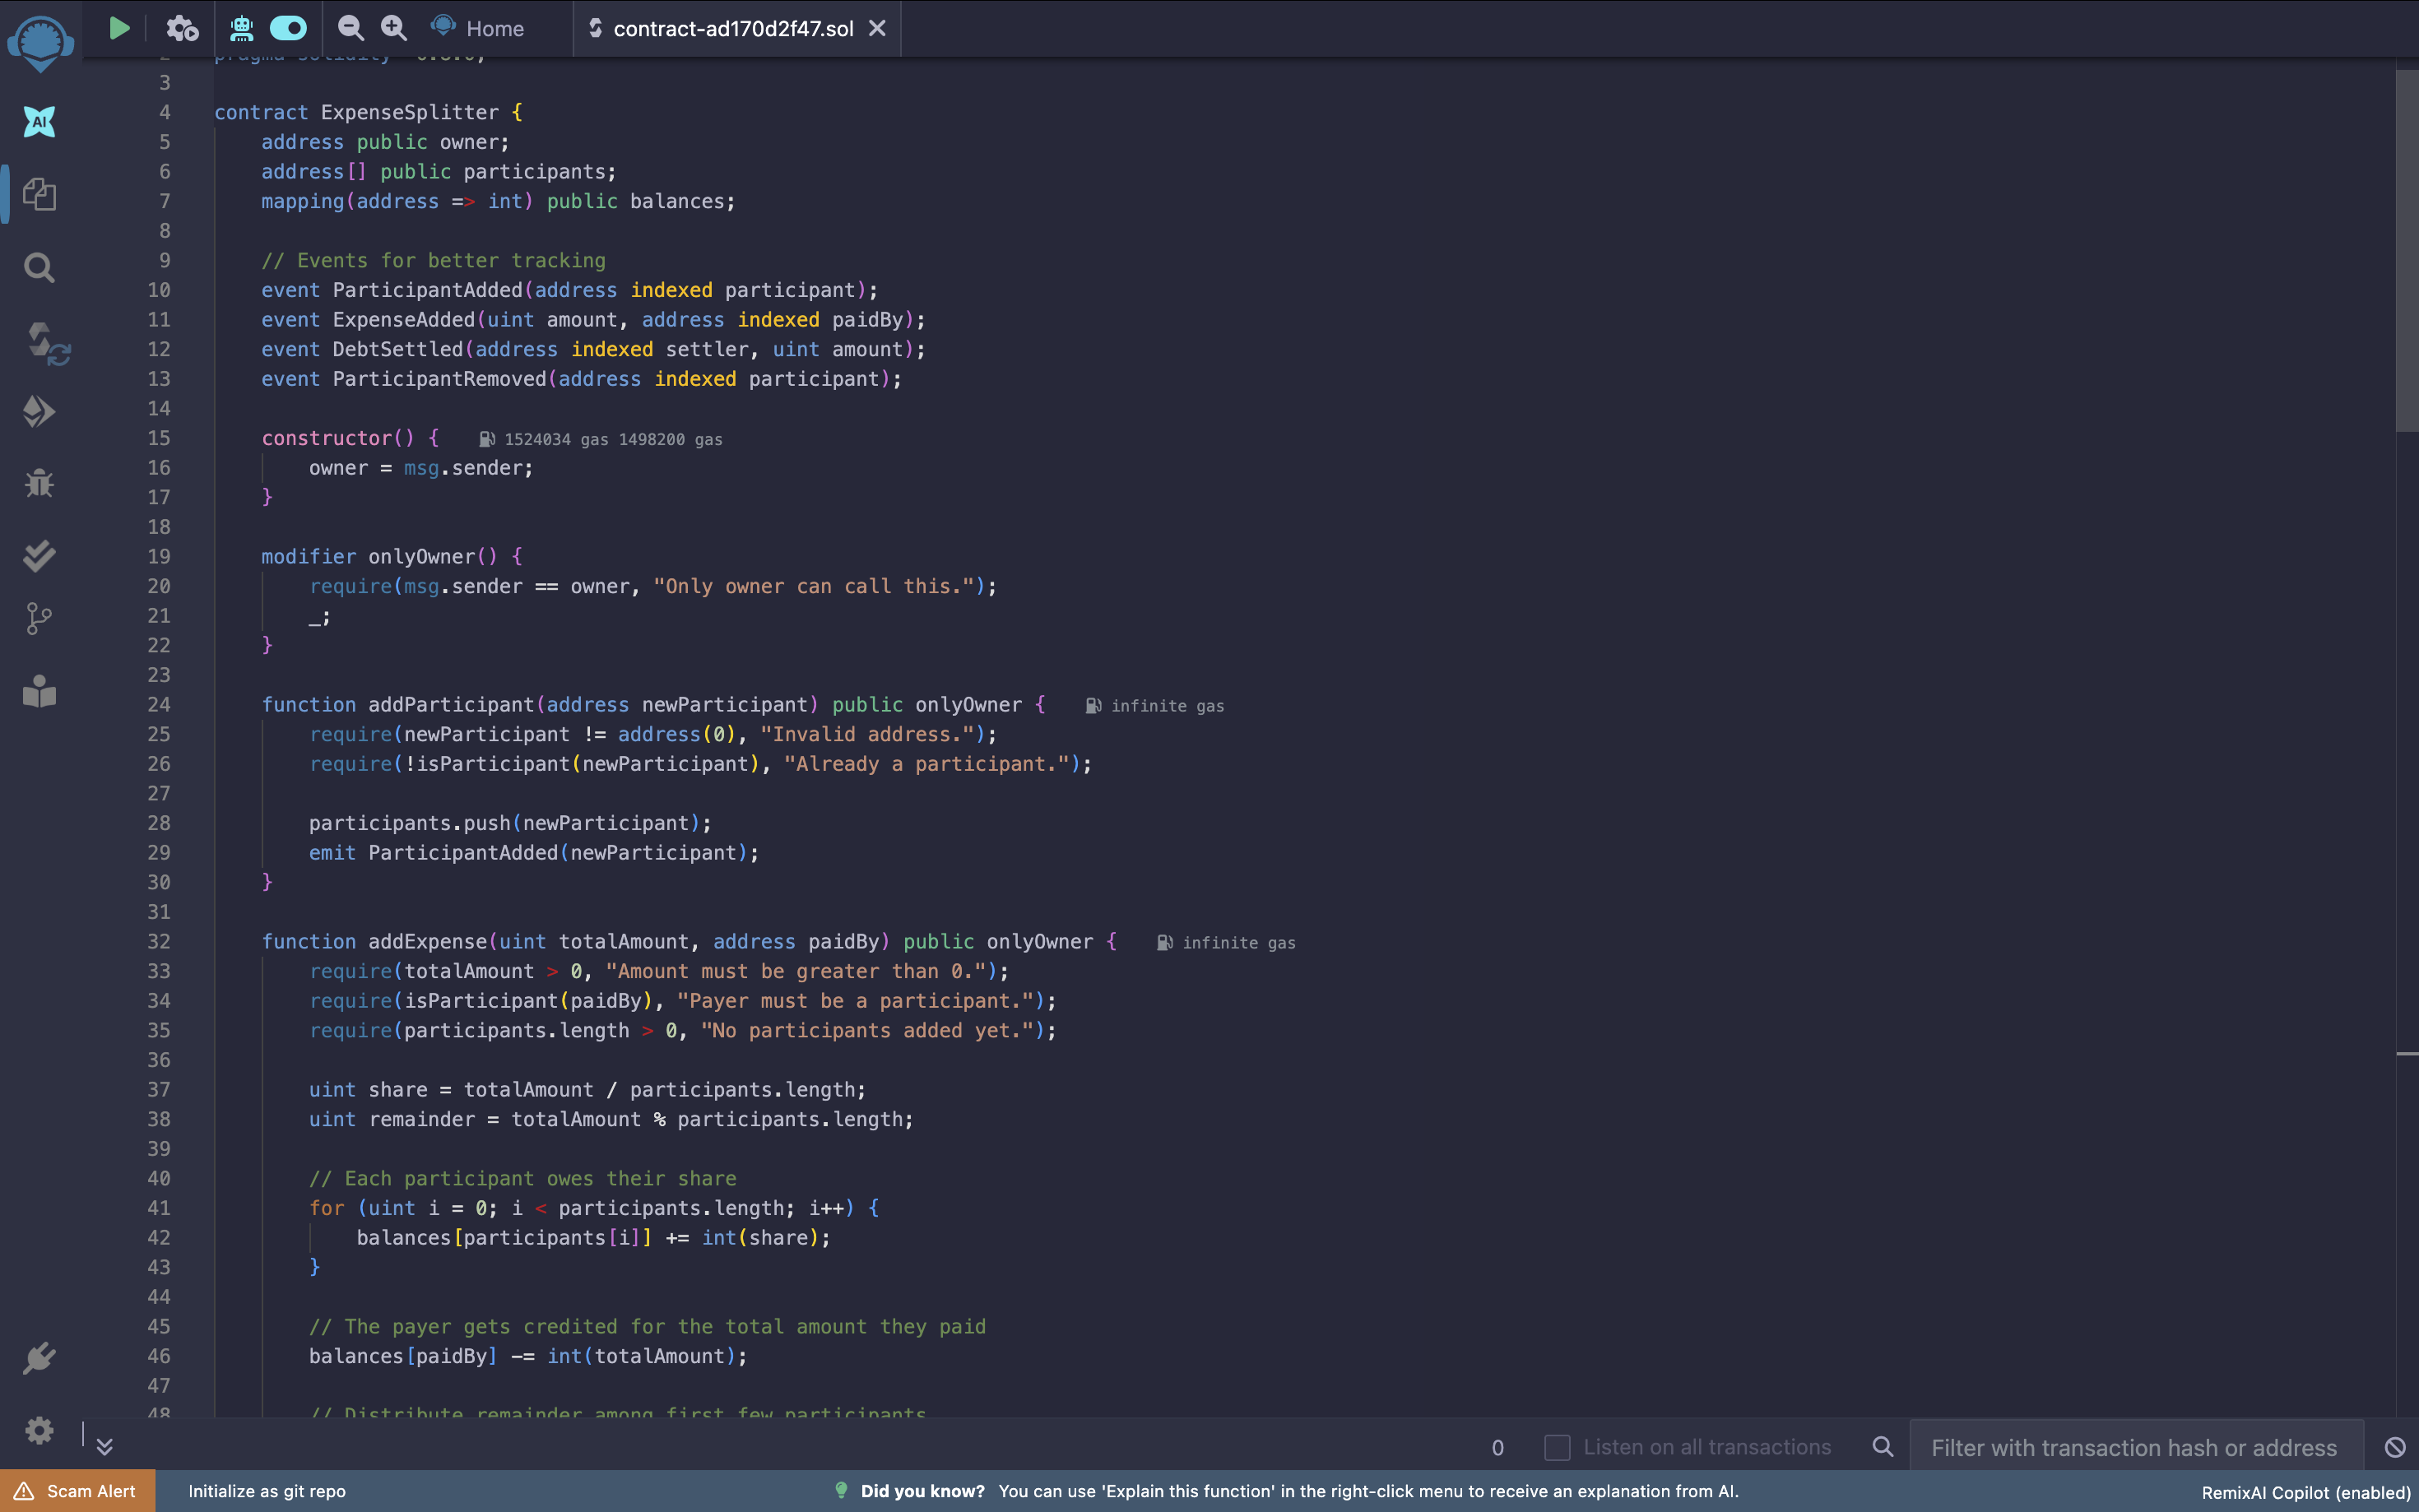
\includegraphics[width=0.6\textwidth]{solidity_example.png}
    \caption{Example of a smart contract workflow in Remix IDE.}
    \label{fig:remix_smart_contract}
\end{figure}
\subsection{Compile the Contract}
After writing the Solidity code, you need to compile the contract. In Remix IDE, this can be done by navigating to the "Solidity Compiler" tab and clicking the "Compile" button. Make sure there are no errors in your code before proceeding.
\subsection{Deploy the Contract}
Once the contract is compiled successfully, you can deploy it to the Ethereum network. In Remix IDE, go to the "Deploy \& Run Transactions" tab, select the appropriate environment (e.g., JavaScript VM, Injected Web3), and click the "Deploy" button.
\textbf{Note:} If you are deploying to a test network or the mainnet, ensure you have a wallet (like MetaMask) connected and sufficient Ether for gas fees.
\subsection{Setup MetaMask Wallet}
To interact with the Ethereum network, you need a wallet. MetaMask is a popular browser extension that allows you to manage your Ethereum accounts and sign transactions. Follow these steps to set up MetaMask:
\begin{itemize}
    \item Install the MetaMask extension for your browser (available for Chrome, Firefox, and Brave).
    \item Create a new wallet or import an existing one using your seed phrase.
    \item Connect MetaMask to the desired Ethereum network (e.g., Mainnet, Ropsten, Rinkeby).
    \item Fund your wallet with test Ether from a faucet if you are using a test network.
\end{itemize}
\begin{figure}[h]
    \centering
    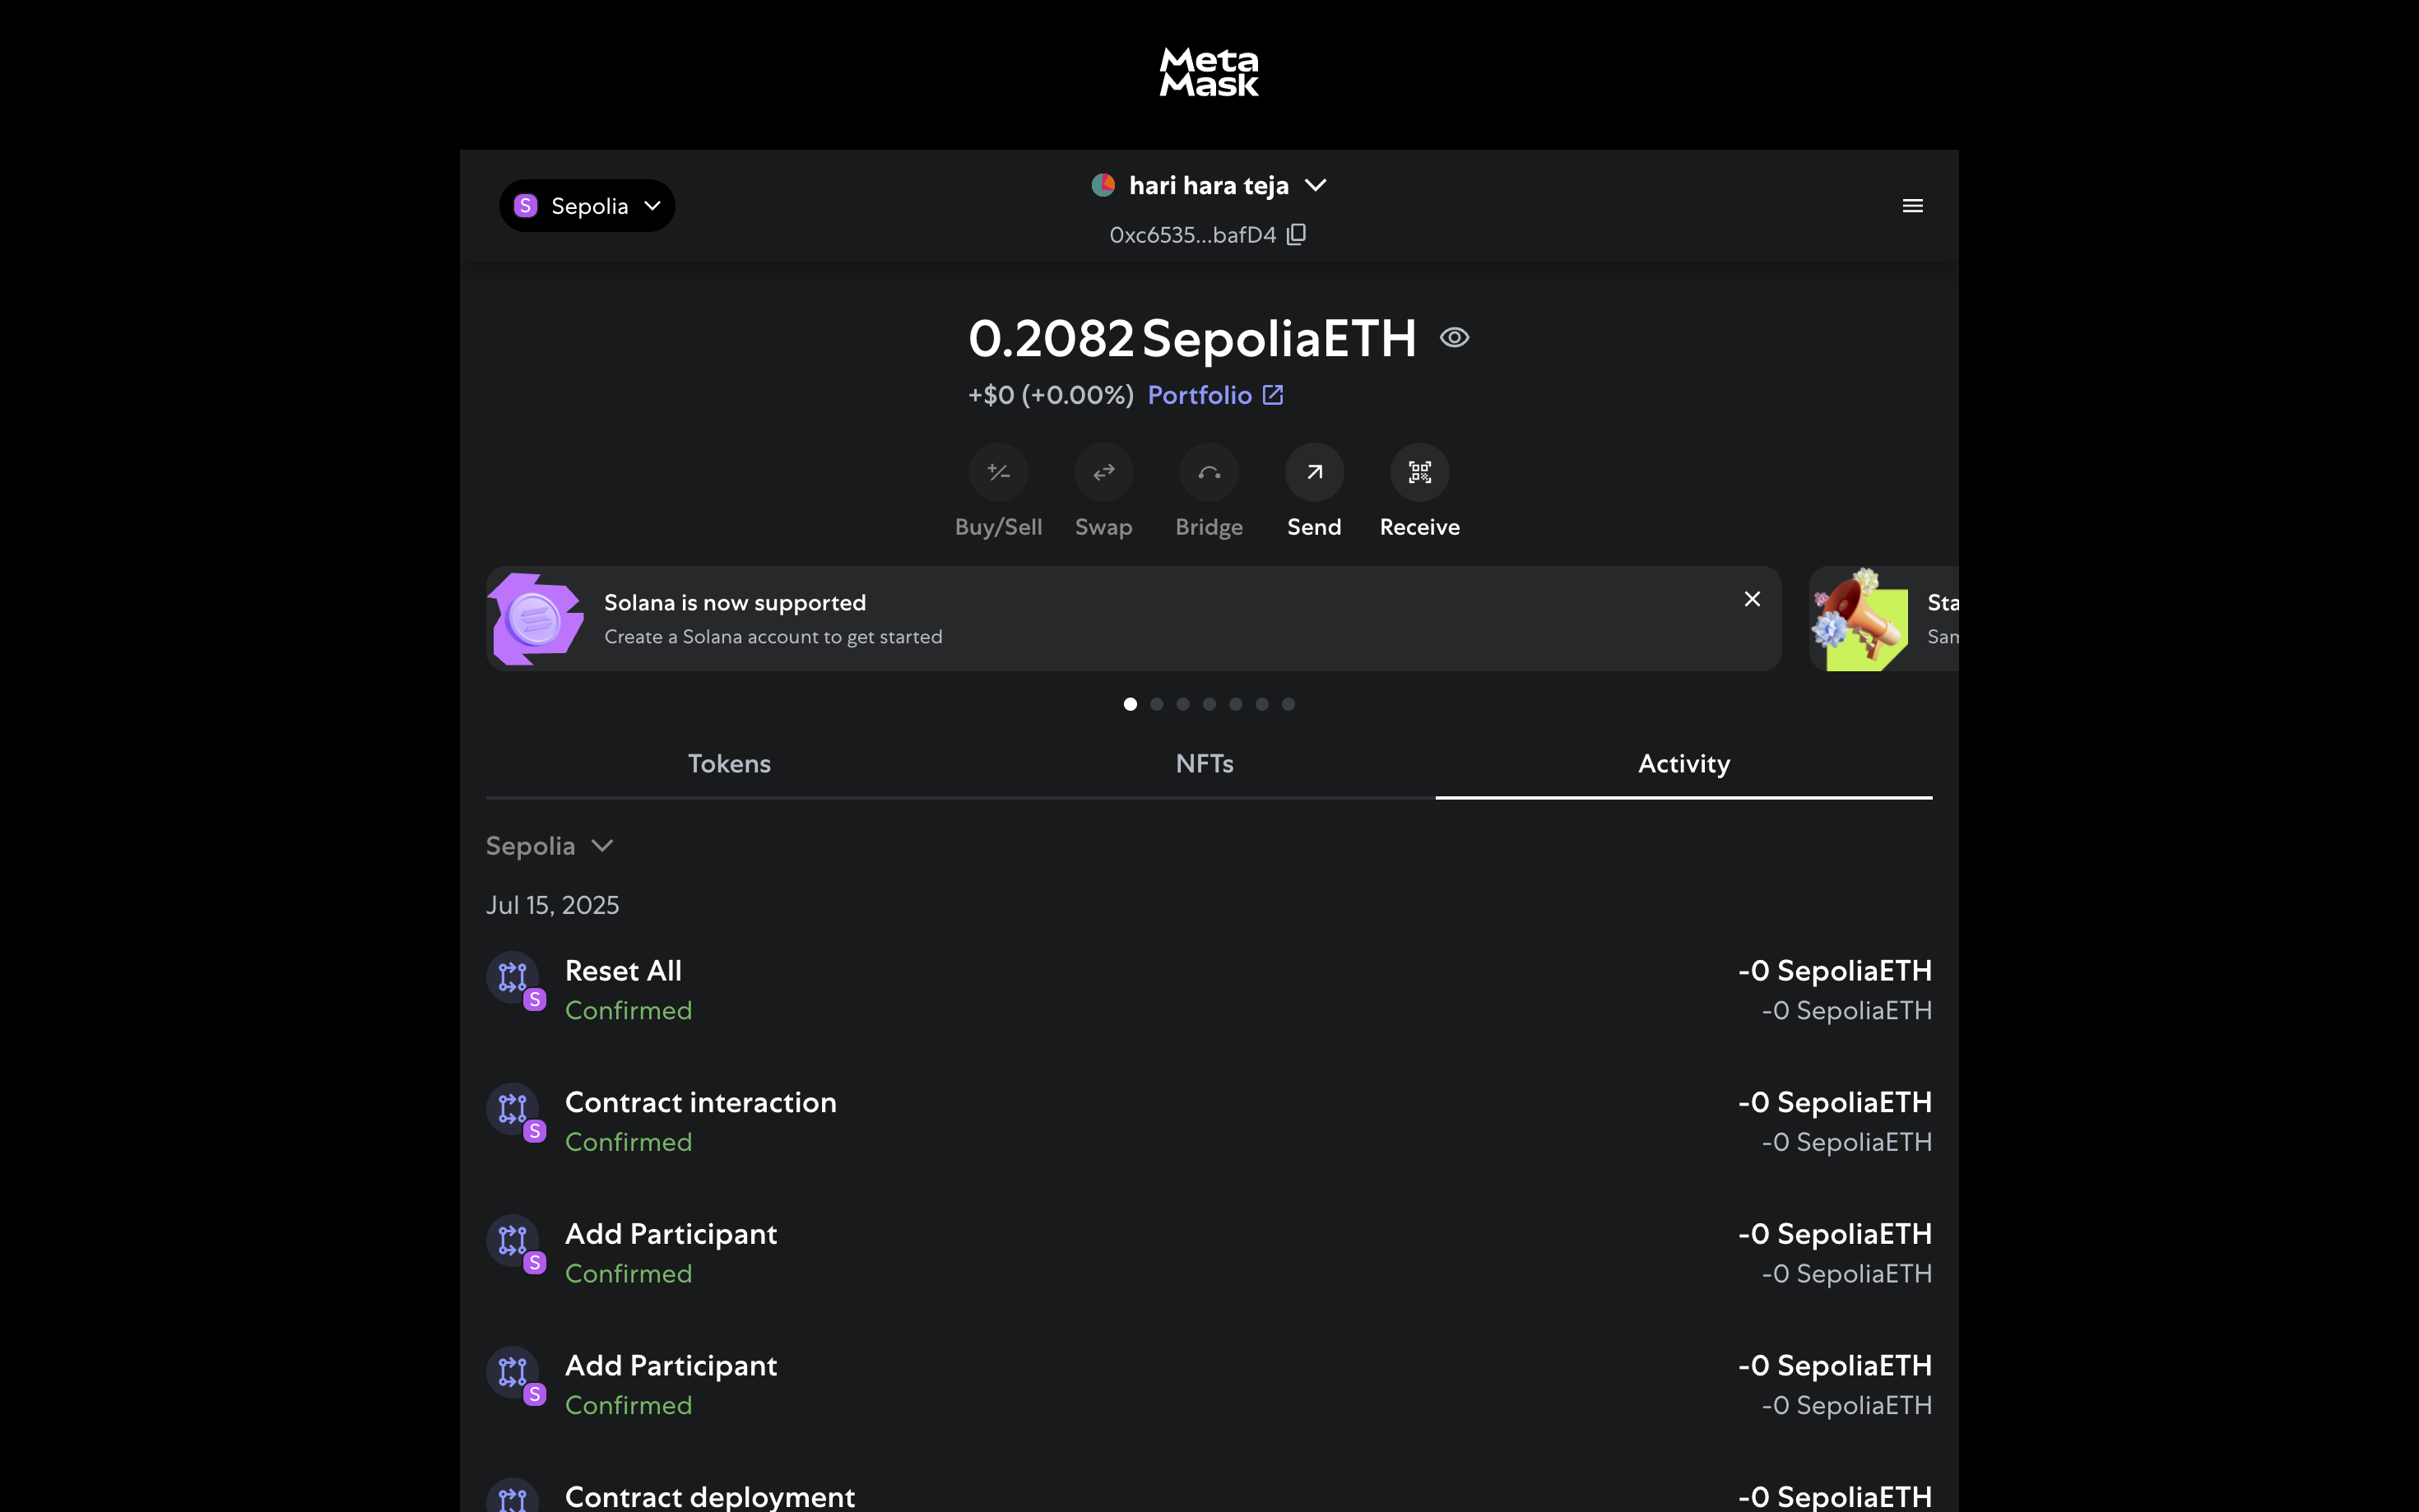
\includegraphics[width=0.6\textwidth]{metamask_setup.png}
    \caption{Setting up MetaMask wallet for Ethereum transactions.}
    \label{fig:metamask_setup}
\end{figure}
\subsection{Connect MetaMask to Remix}
To connect MetaMask to Remix, follow these steps:
\begin{itemize}
    \item In Remix IDE, go to the "Deploy and Run Transactions" tab.
    \item Select "Injected Web3" as the environment.
    \item MetaMask will prompt you to connect your wallet. Approve the connection.
    \item Once connected, you will see your MetaMask account address in the Remix interface.
\end{itemize}
\subsection{Compile the Contract}
After writing the Solidity code, you need to compile the contract. In Remix IDE, this can be done by navigating to the "Solidity Compiler" tab and clicking the "Compile" button. Make sure there are no errors in your code before proceeding.
\subsection{Deploy the Contract}
Once the contract is compiled successfully, you can deploy it to the Ethereum network. In Remix IDE, go to the "Deploy \& Run Transactions" tab, select the appropriate environment (e.g., JavaScript VM, Injected Web3), and click the "Deploy" button.
\textbf{Note:} If you are deploying to a test network or the mainnet, ensure you have a wallet (like MetaMask) connected and sufficient Ether for gas fees.
\subsection{Interact with the Contract}
After deploying the contract, you can interact with it through the Remix interface. You can call functions, send transactions, and view the contract's state. For example, if your contract has a function to set a value, you can enter the value in the input field and click the corresponding button to execute the function. The transaction will be sent to the Ethereum network, and you can view the transaction details in the Remix console or your MetaMask wallet.
\subsection{Verify the Contract}
After deploying the contract, it is a good practice to verify it on Etherscan or similar block explorers. Verification allows others to view the source code and understand the contract's functionality. To verify the contract, you can use the "Verify Contract" feature on Etherscan by providing the contract address and the Solidity source code. This step is optional but recommended for transparency and trustworthiness.    
\section{ExampleContract}
\begin{verbatim}
pragma solidity ^0.8.0;

// SPDX-License-Identifier: MIT

// This contract demonstrates key Solidity concepts: variables, functions, modifiers, events, storage/memory, inheritance, and interfaces.

interface ICounter {
    function getCount() external view returns (uint256);
}

contract Ownable {
    address public owner;

    constructor() {
        owner = msg.sender;
    }

    modifier onlyOwner() {
        require(msg.sender == owner, "Not the owner");
        _;
    }
}

contract ExampleContract is Ownable, ICounter {
    // State variables
    uint256 public count;
    string public name;
    mapping(address => uint256) public balances;

    // Event declaration
    event CountIncremented(uint256 newCount, address indexed by);
    event NameChanged(string oldName, string newName);

    // Constructor
    constructor(string memory _name) {
        name = _name;
    }

    // Public function to increment count
    function increment() public {
        count += 1;
        emit CountIncremented(count, msg.sender);
    }

    // External function to get count (implements interface)
    function getCount() external view override returns (uint256) {
        return count;
    }

    // Function with onlyOwner modifier
    function setName(string memory _newName) public onlyOwner {
        emit NameChanged(name, _newName);
        name = _newName;
    }

    // Pure function (does not read or modify state)
    function add(uint256 a, uint256 b) public pure returns (uint256) {
        return a + b;
    }

    // View function (reads state, does not modify)
    function getBalance(address user) public view returns (uint256) {
        return balances[user];
    }

    // Function demonstrating storage vs memory
    function updateBalance(address user, uint256 amount) public {
        balances[user] = amount; // storage
    }

    // Internal function
    function _resetCount() internal {
        count = 0;
    }

    // Private function
    function _secret() private pure returns (string memory) {
        return "This is private";
    }
}
\end{verbatim}
\subsection{Explanation of ExampleContract}
The `ExampleContract` demonstrates various Solidity concepts:
\begin{itemize}
    \item State Variables: `count`, `name`, and `balances` are stored on the blockchain.
    \item Events: `CountIncremented` and `NameChanged` are emitted to log important actions.
    \item Modifiers: `onlyOwner` restricts access to certain functions, ensuring only the contract owner can call them.
    \item Functions: Includes public, external, pure, and view functions to interact with the contract.
    \item Inheritance: Inherits from `Ownable` for ownership management and implements the `ICounter` interface to provide a standardized way to get the count.
    \item Storage vs Memory: Demonstrates the difference between storage (persistent on the blockchain) and memory (temporary during function execution).
\end{itemize}
\section{How smart contracts connect with the frontend}
Smart contracts connect with the frontend through libraries like ethers.js or web3.js, which provide APIs to interact with the Ethereum blockchain. The frontend, built using frameworks like React or Vue.js, communicates with the smart contract by sending transactions, reading data, and listening for events. Users can interact with the smart contract through a user interface, allowing them to perform actions like sending transactions, querying balances, and executing functions defined in the smart contract. The frontend also handles wallet connections (e.g., MetaMask) to enable users to sign transactions and manage their Ethereum accounts. This integration allows for a seamless user experience, bridging the gap between the blockchain and the web application.
\subsection{introduction to web3.js}
Web3.js is a popular JavaScript library that allows developers to interact with the Ethereum blockchain. It provides a convenient API for sending transactions, interacting with smart contracts, and querying blockchain data. Web3.js abstracts away the complexities of dealing with the Ethereum JSON-RPC API, making it easier for developers to build decentralized applications (dApps). With Web3.js, developers can connect to various Ethereum networks (e.g., mainnet, testnets) and work with different Ethereum-compatible wallets. The library is commonly used in conjunction with frontend frameworks like React and Vue.js to create responsive and user-friendly dApps.
\subsection{introduction to ethers.js}
Ethers.js is another popular JavaScript library for interacting with the Ethereum blockchain. It is designed to be a lightweight and easy-to-use alternative to Web3.js, providing a simple API for common tasks like sending transactions, interacting with smart contracts, and querying blockchain data. Ethers.js emphasizes security and developer experience, with features like built-in TypeScript support and a focus on immutability. The library also includes a wallet implementation, allowing developers to manage user accounts and sign transactions directly within their applications. Ethers.js is often used in modern dApp development, particularly in conjunction with frameworks like React and Vue.js. 
\subsection{Requirements for running the frontend locally}
To run the frontend locally, you will need the following:
\begin{itemize}
    \item Node.js: Ensure you have Node.js installed on your machine. You can download it from [nodejs.org](https://nodejs.org/).
    \item Package Manager: Use npm (comes with Node.js) or yarn to manage dependencies.
    \item Frontend Framework: Choose a framework like React or Vue.js for building the user interface.
    \item Ethereum Wallet: Install a wallet like MetaMask to interact with the Ethereum blockchain.
    \item Local Blockchain: Optionally, set up a local Ethereum blockchain using tools like Ganache for testing purposes.
\end{itemize}
\subsection{Running the frontend locally}
\begin{itemize}
  \item \textbf{ReactJS}: For creating the frontend interface.
  \item \textbf{Web3.js}: To interact with the smart contract and blockchain.
  \item \textbf{MetaMask}: Ethereum wallet to manage user accounts and sign transactions.
  \item \textbf{ABI (Application Binary Interface)}: Describes the structure of smart contract functions.
\end{itemize}

\subsection*{Getting the ABI}
\begin{itemize}
  \item \textbf{Using Remix IDE:}
    \begin{itemize}
      \item Click on the \texttt{Compilation} tab.
      \item Compile your \texttt{.sol} file.
      \item Go to the \texttt{Deploy \& Run Transactions} tab.
      \item Scroll down and find the contract section.
      \item Click the \textbf{ABI} button or copy it from the JSON box.
    \end{itemize}
  \item \textbf{Using Hardhat or Truffle:}
    \begin{itemize}
      \item After compiling, go to \texttt{artifacts} or \texttt{build/contracts} folder.
      \item Open the generated \texttt{.json} file.
      \item Copy the \texttt{"abi"} field.
    \end{itemize}
\end{itemize}

\section{Steps to Connect Frontend with Smart Contract}

\subsection{Install Web3.js}
\begin{verbatim}
npm install web3
\end{verbatim}

\subsection{Import Web3 in React}
\begin{verbatim}
import Web3 from 'web3';
\end{verbatim}

\subsection{Initialize Web3 and Request Accounts}
\begin{verbatim}
const web3 = new Web3(window.ethereum);
const accounts = await window.ethereum.request({ method: 'eth_requestAccounts' });
const account = accounts[0];
\end{verbatim}

\subsection{Connect to Smart Contract}
\begin{verbatim}
const contract = new web3.eth.Contract(contractABI, contractAddress);
\end{verbatim}

\subsection{Interact with Smart Contract}
\textbf{Read Data:}
\begin{verbatim}
const result = await contract.methods.getData().call();
\end{verbatim}

\textbf{Write Data:}
\begin{verbatim}
await contract.methods.setData("value").send({ from: account });
\end{verbatim}

\subsection{MetaMask Integration}
Ensure that MetaMask is installed and connected. MetaMask injects the \texttt{window.ethereum} object, which Web3 uses to communicate with the Ethereum blockchain.

You can also listen to account and network changes:
\begin{verbatim}
window.ethereum.on("accountsChanged", handleAccountsChanged);
window.ethereum.on("chainChanged", handleChainChanged);
\end{verbatim}

\subsection{Conclusion}
Web3.js serves as a bridge between the frontend and blockchain. By using React, Web3.js, and MetaMask together, developers can build interactive decentralized applications where users can send transactions and view real-time data from the Ethereum network.
\section{A Mini Project - Decentralized Expense Splitter}
\subsection{Project Overview}
The Expense Splitter DApp is a decentralized application designed to simplify group expense management using blockchain technology. It allows a group of participants to track shared expenses, compute individual balances, and settle debts transparently. Built on the Ethereum blockchain, the backend of the application is powered by a Solidity smart contract that handles participant registration, expense distribution, and balance calculation. Each expense is split evenly among participants, and the smart contract keeps track of who owes what.
\newline
The frontend is developed using React and styled with Tailwind CSS for a modern and responsive user experience. Ethers.js is used to connect the frontend to the Ethereum network, enabling wallet integration via MetaMask, real-time balance fetching, and secure transaction submission. The app features animated UI components using Framer Motion, wallet connection cards, and dynamic balance displays. Users can add expenses in ETH (automatically converted to Wei under the hood), view participant balances, and settle their debts with a single click.
\newpage

\subsection{Smart Contract Code}
\begin{verbatim}
    // SPDX-License-Identifier: MIT
    pragma solidity ^0.8.0;

    contract ExpenseSplitter {
        address public owner;
        address[] public participants;
        mapping(address => int) public balances;
        
        // Events for better tracking
        event ParticipantAdded(address indexed participant);
        event ExpenseAdded(uint amount, address indexed paidBy);
        event DebtSettled(address indexed settler, uint amount);
        event ParticipantRemoved(address indexed participant);
        
        constructor() {
            owner = msg.sender;
        }
        
        modifier onlyOwner() {
            require(msg.sender == owner, "Only owner can call this.");
            _;
        }
        
        function addParticipant(address newParticipant) public onlyOwner {
            require(newParticipant != address(0), "Invalid address.");
            require(!isParticipant(newParticipant), "Already a participant.");
            
            participants.push(newParticipant);
            emit ParticipantAdded(newParticipant);
        }
        
        function addExpense(uint totalAmount, address paidBy) public onlyOwner {
            require(totalAmount > 0, "Amount must be greater than 0.");
            require(isParticipant(paidBy), "Payer must be a participant.");
            require(participants.length > 0, "No participants added yet.");
            
            uint share = totalAmount / participants.length;
            uint remainder = totalAmount % participants.length;
            
            // Each participant owes their share
            for (uint i = 0; i < participants.length; i++) {
                balances[participants[i]] += int(share);
            }
            
            // The payer gets credited for the total amount they paid
            balances[paidBy] -= int(totalAmount);
            
            // Distribute remainder among first few participants
            for (uint i = 0; i < remainder; i++) {
                balances[participants[i]] += 1;
            }
            
            emit ExpenseAdded(totalAmount, paidBy);
        }
        
        // function settle() removed due to duplication
        
        function getBalance(address user) public view returns (int) {
            return balances[user];
        }
        
        function getParticipantsCount() public view returns (uint) {
            return participants.length;
        }
        
        function getParticipant(uint index) public view returns (address) {
            require(index < participants.length, "Index out of bounds");
            return participants[index];
        }
        
        function isParticipant(address user) public view returns (bool) {
            for (uint i = 0; i < participants.length; i++) {
                if (participants[i] == user) {
                    return true;
                }
            }
            return false;
        }
        
        // Additional utility functions
        function getAllParticipants() public view returns (address[] memory) {
            return participants;
        }
        
        function getAllBalances() public view returns (address[] memory addresses, int[] memory balanceValues) {
            uint len = participants.length;
            addresses = new address[](len);
            balanceValues = new int[](len);
            
            for (uint i = 0; i < len; i++) {
                addresses[i] = participants[i];
                balanceValues[i] = balances[participants[i]];
            }
        }
        
        function settle() public payable {
                require(balances[msg.sender] > 0, "No debt to settle.");
                require(msg.value == uint(balances[msg.sender]), "Send exact amount.");

                uint amountToSettle = uint(balances[msg.sender]);
                balances[msg.sender] = 0;

                // Transfer to owner
                payable(owner).transfer(msg.value);

                // Decrease owner's negative balance
                balances[owner] -= int(amountToSettle);  // New line

                emit DebtSettled(msg.sender, amountToSettle);
            }
        
        // Emergency function to allow owner to withdraw contract balance
        function emergencyWithdraw() public onlyOwner {
            payable(owner).transfer(address(this).balance);
        }
        
        // Function to check total contract balance
        function getContractBalance() public view returns (uint) {
            return address(this).balance;
        }
        function resetAll() public onlyOwner {
        for (uint i = 0; i < participants.length; i++) {
            balances[participants[i]] = 0;
        }
        delete participants;
    }
    }
\end{verbatim}
\begin{figure}[h]
    \centering
    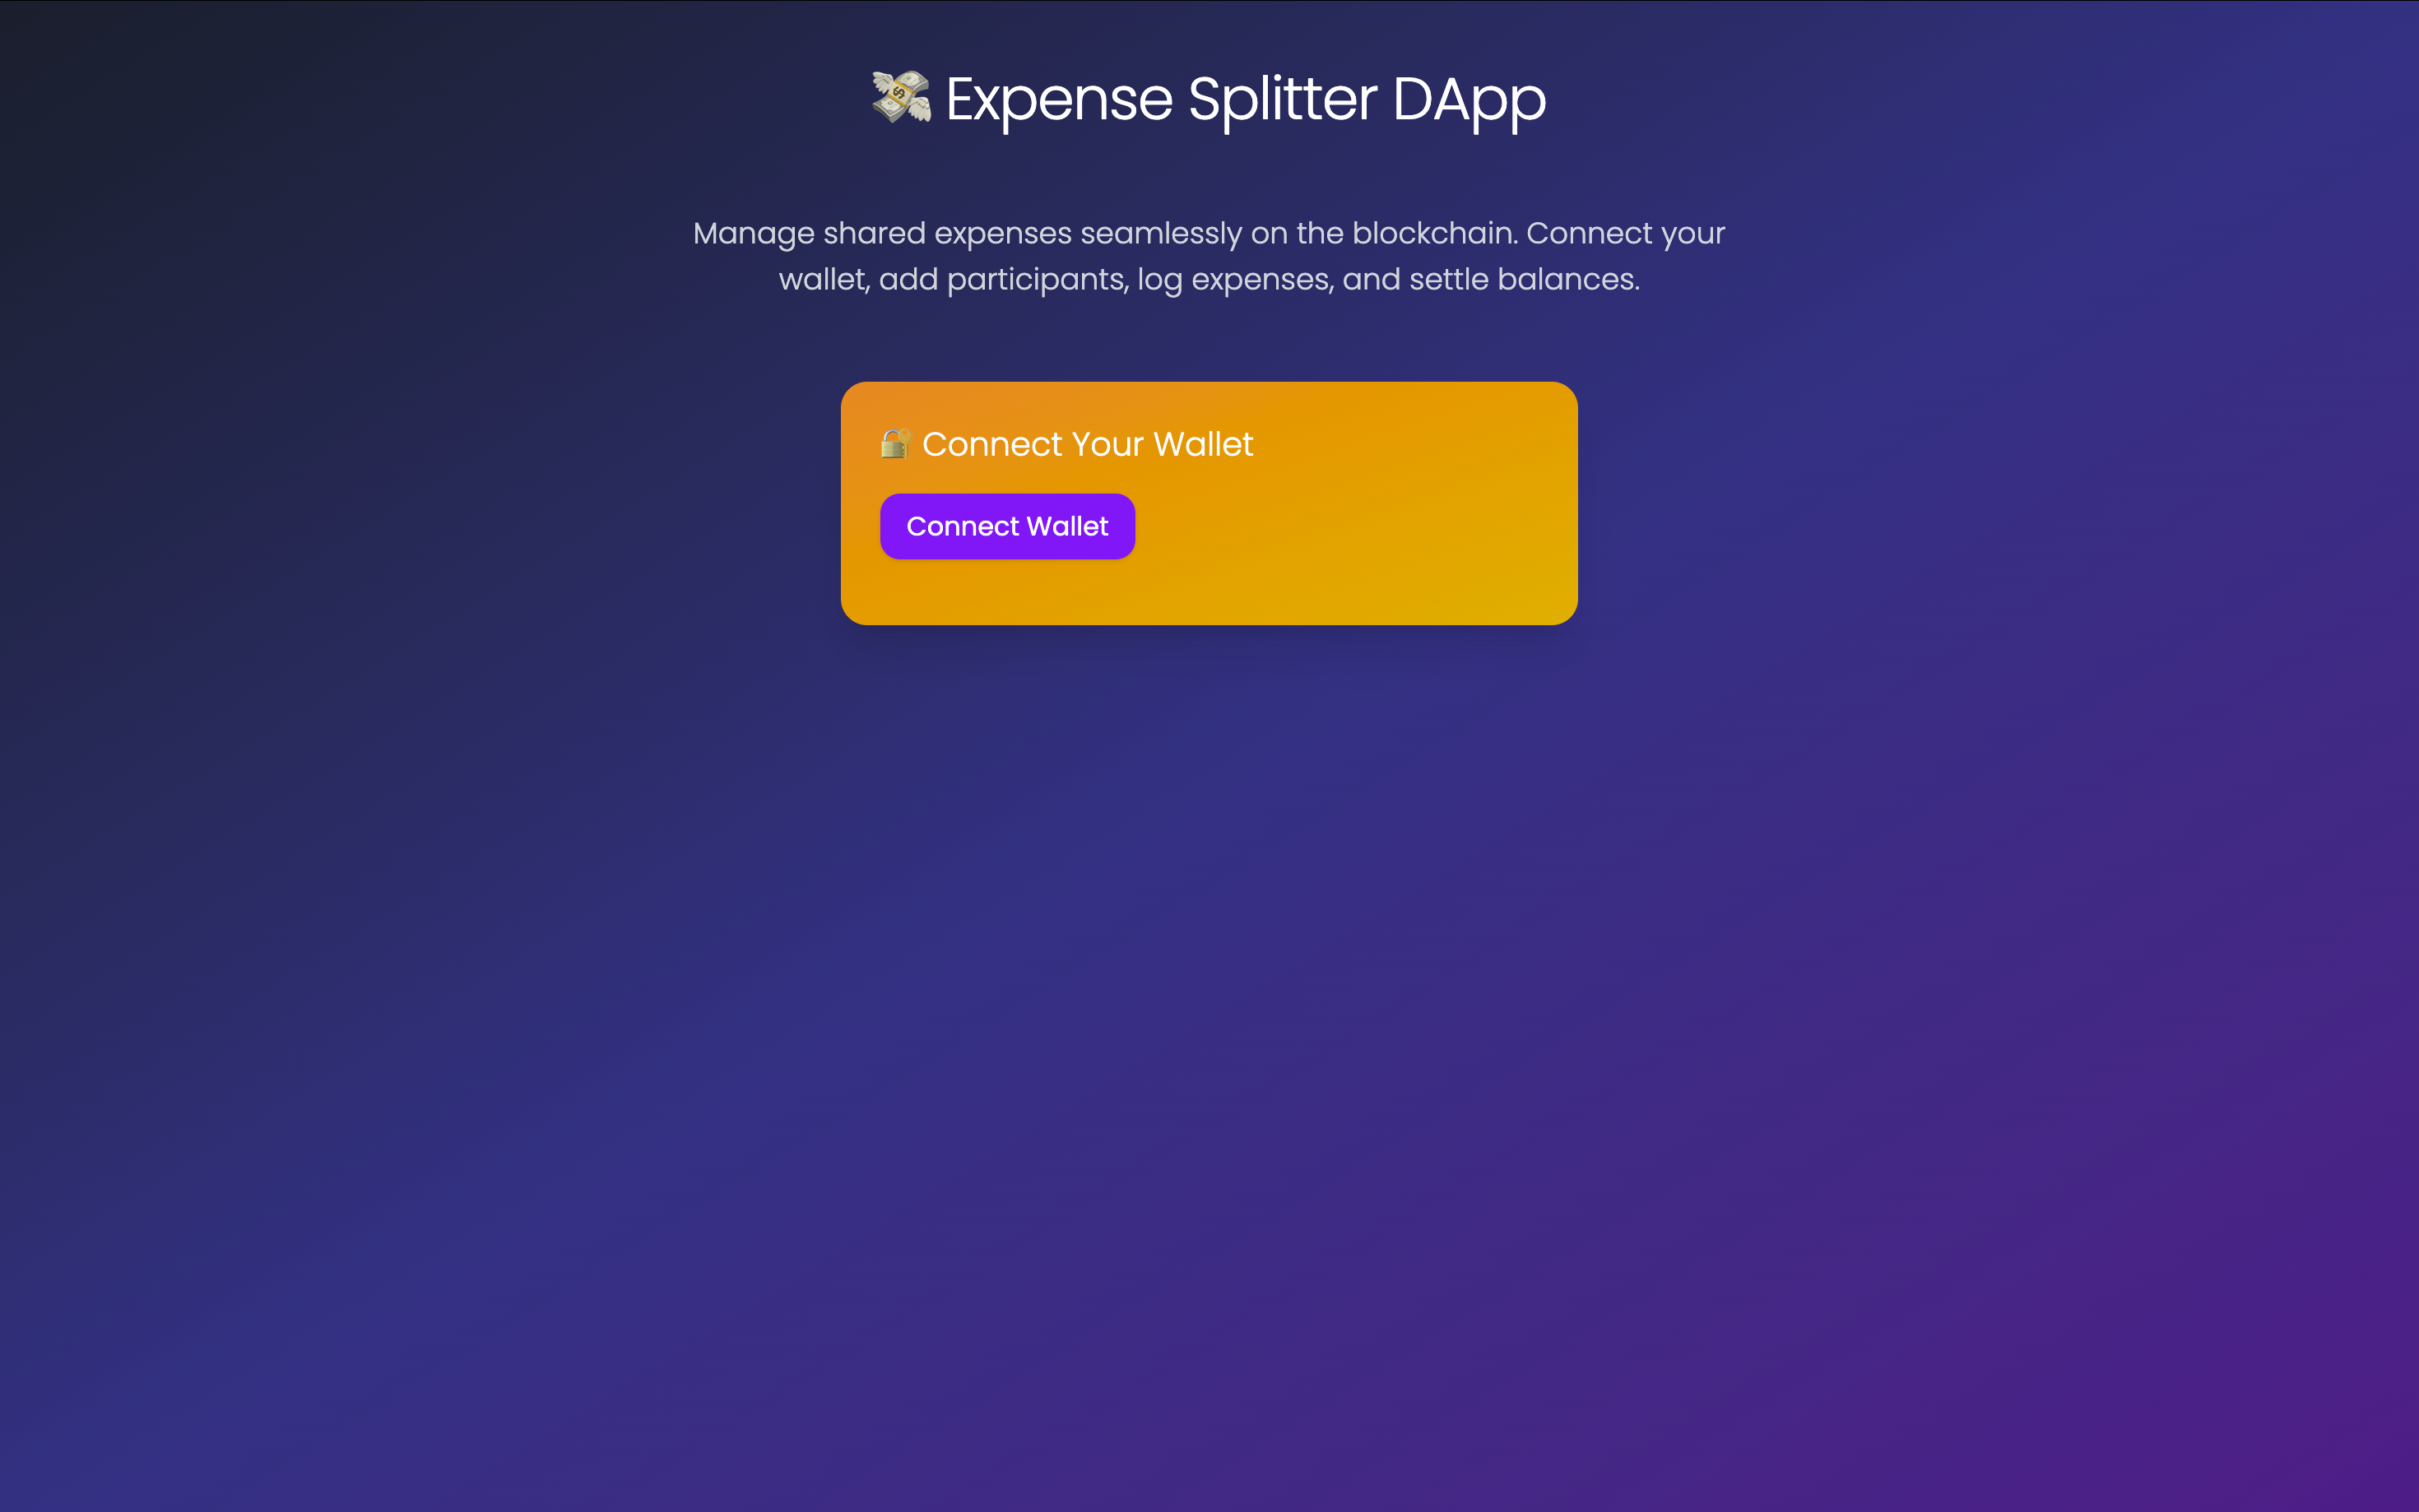
\includegraphics[width=0.7\textwidth]{connect-wallet.png}
    \caption{Connect wallet to Decentralized Expense Splitter DApp.}
    \label{fig:expense_splitter_architecture}
\end{figure}
\begin{figure}[h]
    \centering
    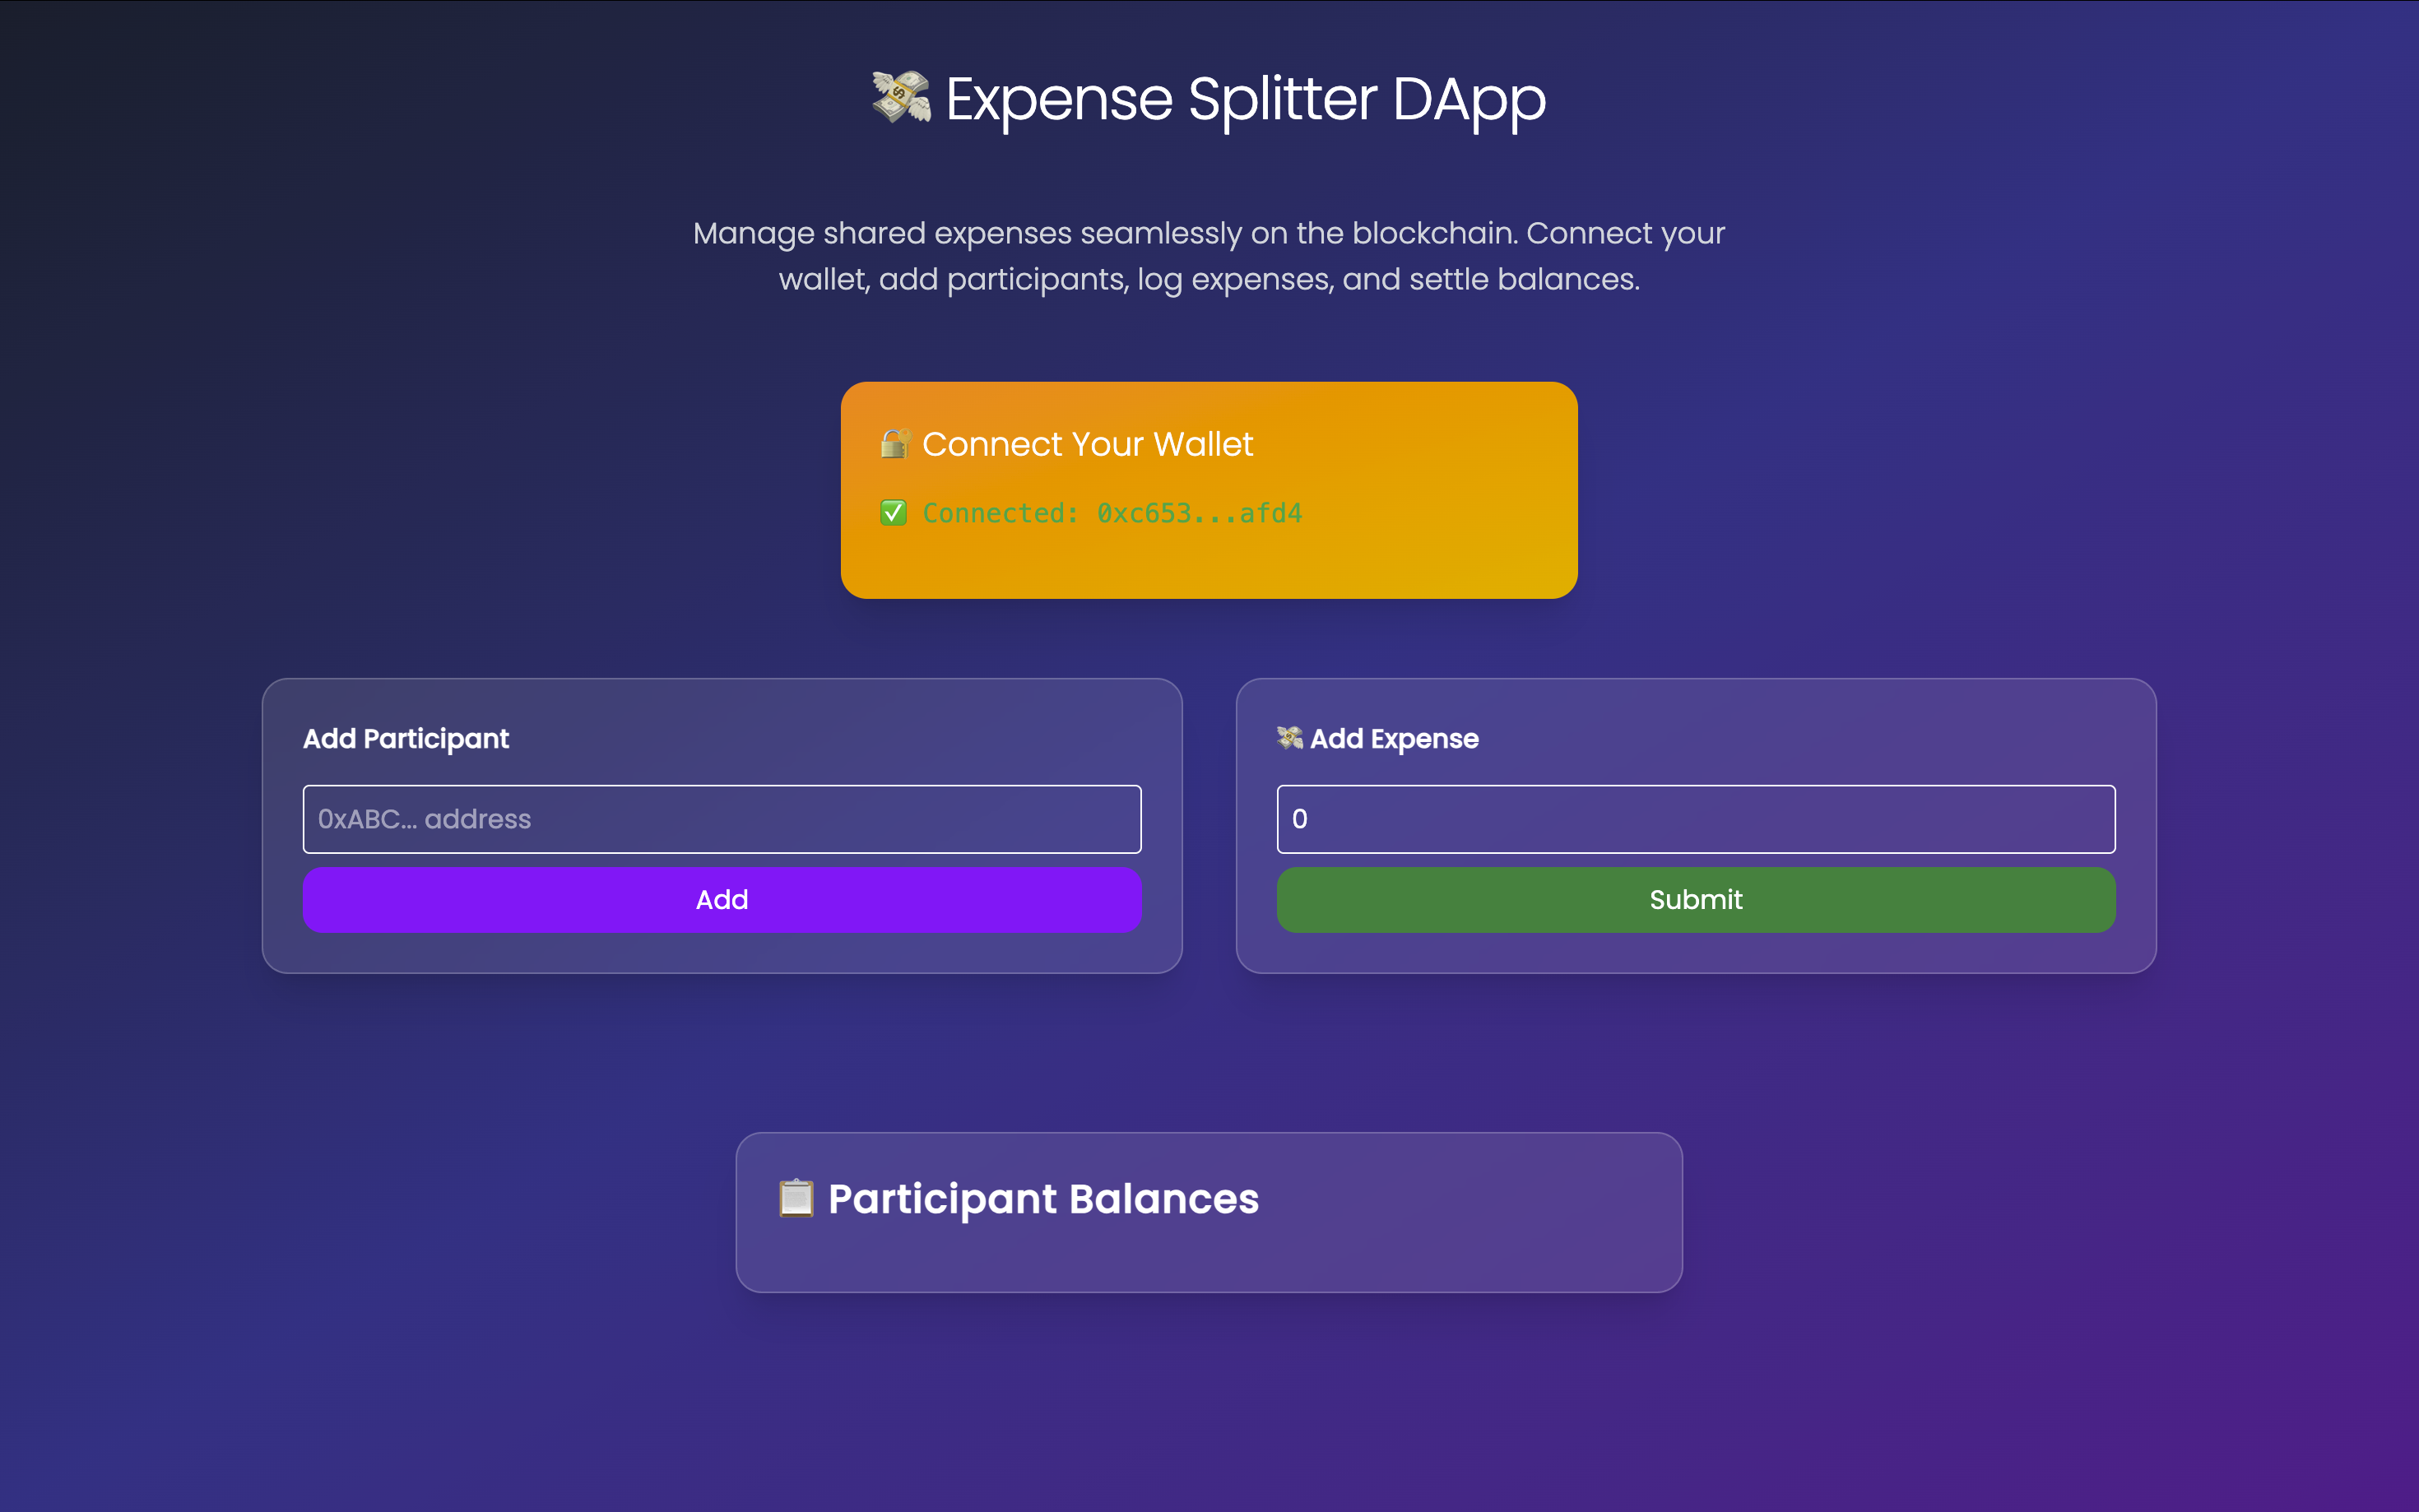
\includegraphics[width=0.7\textwidth]{add_participant.png}
    \caption{Add participants to Decentralized Expense Splitter DApp.}
    \label{fig:add_participants}
\end{figure}
\begin{figure}[h]
    \centering
    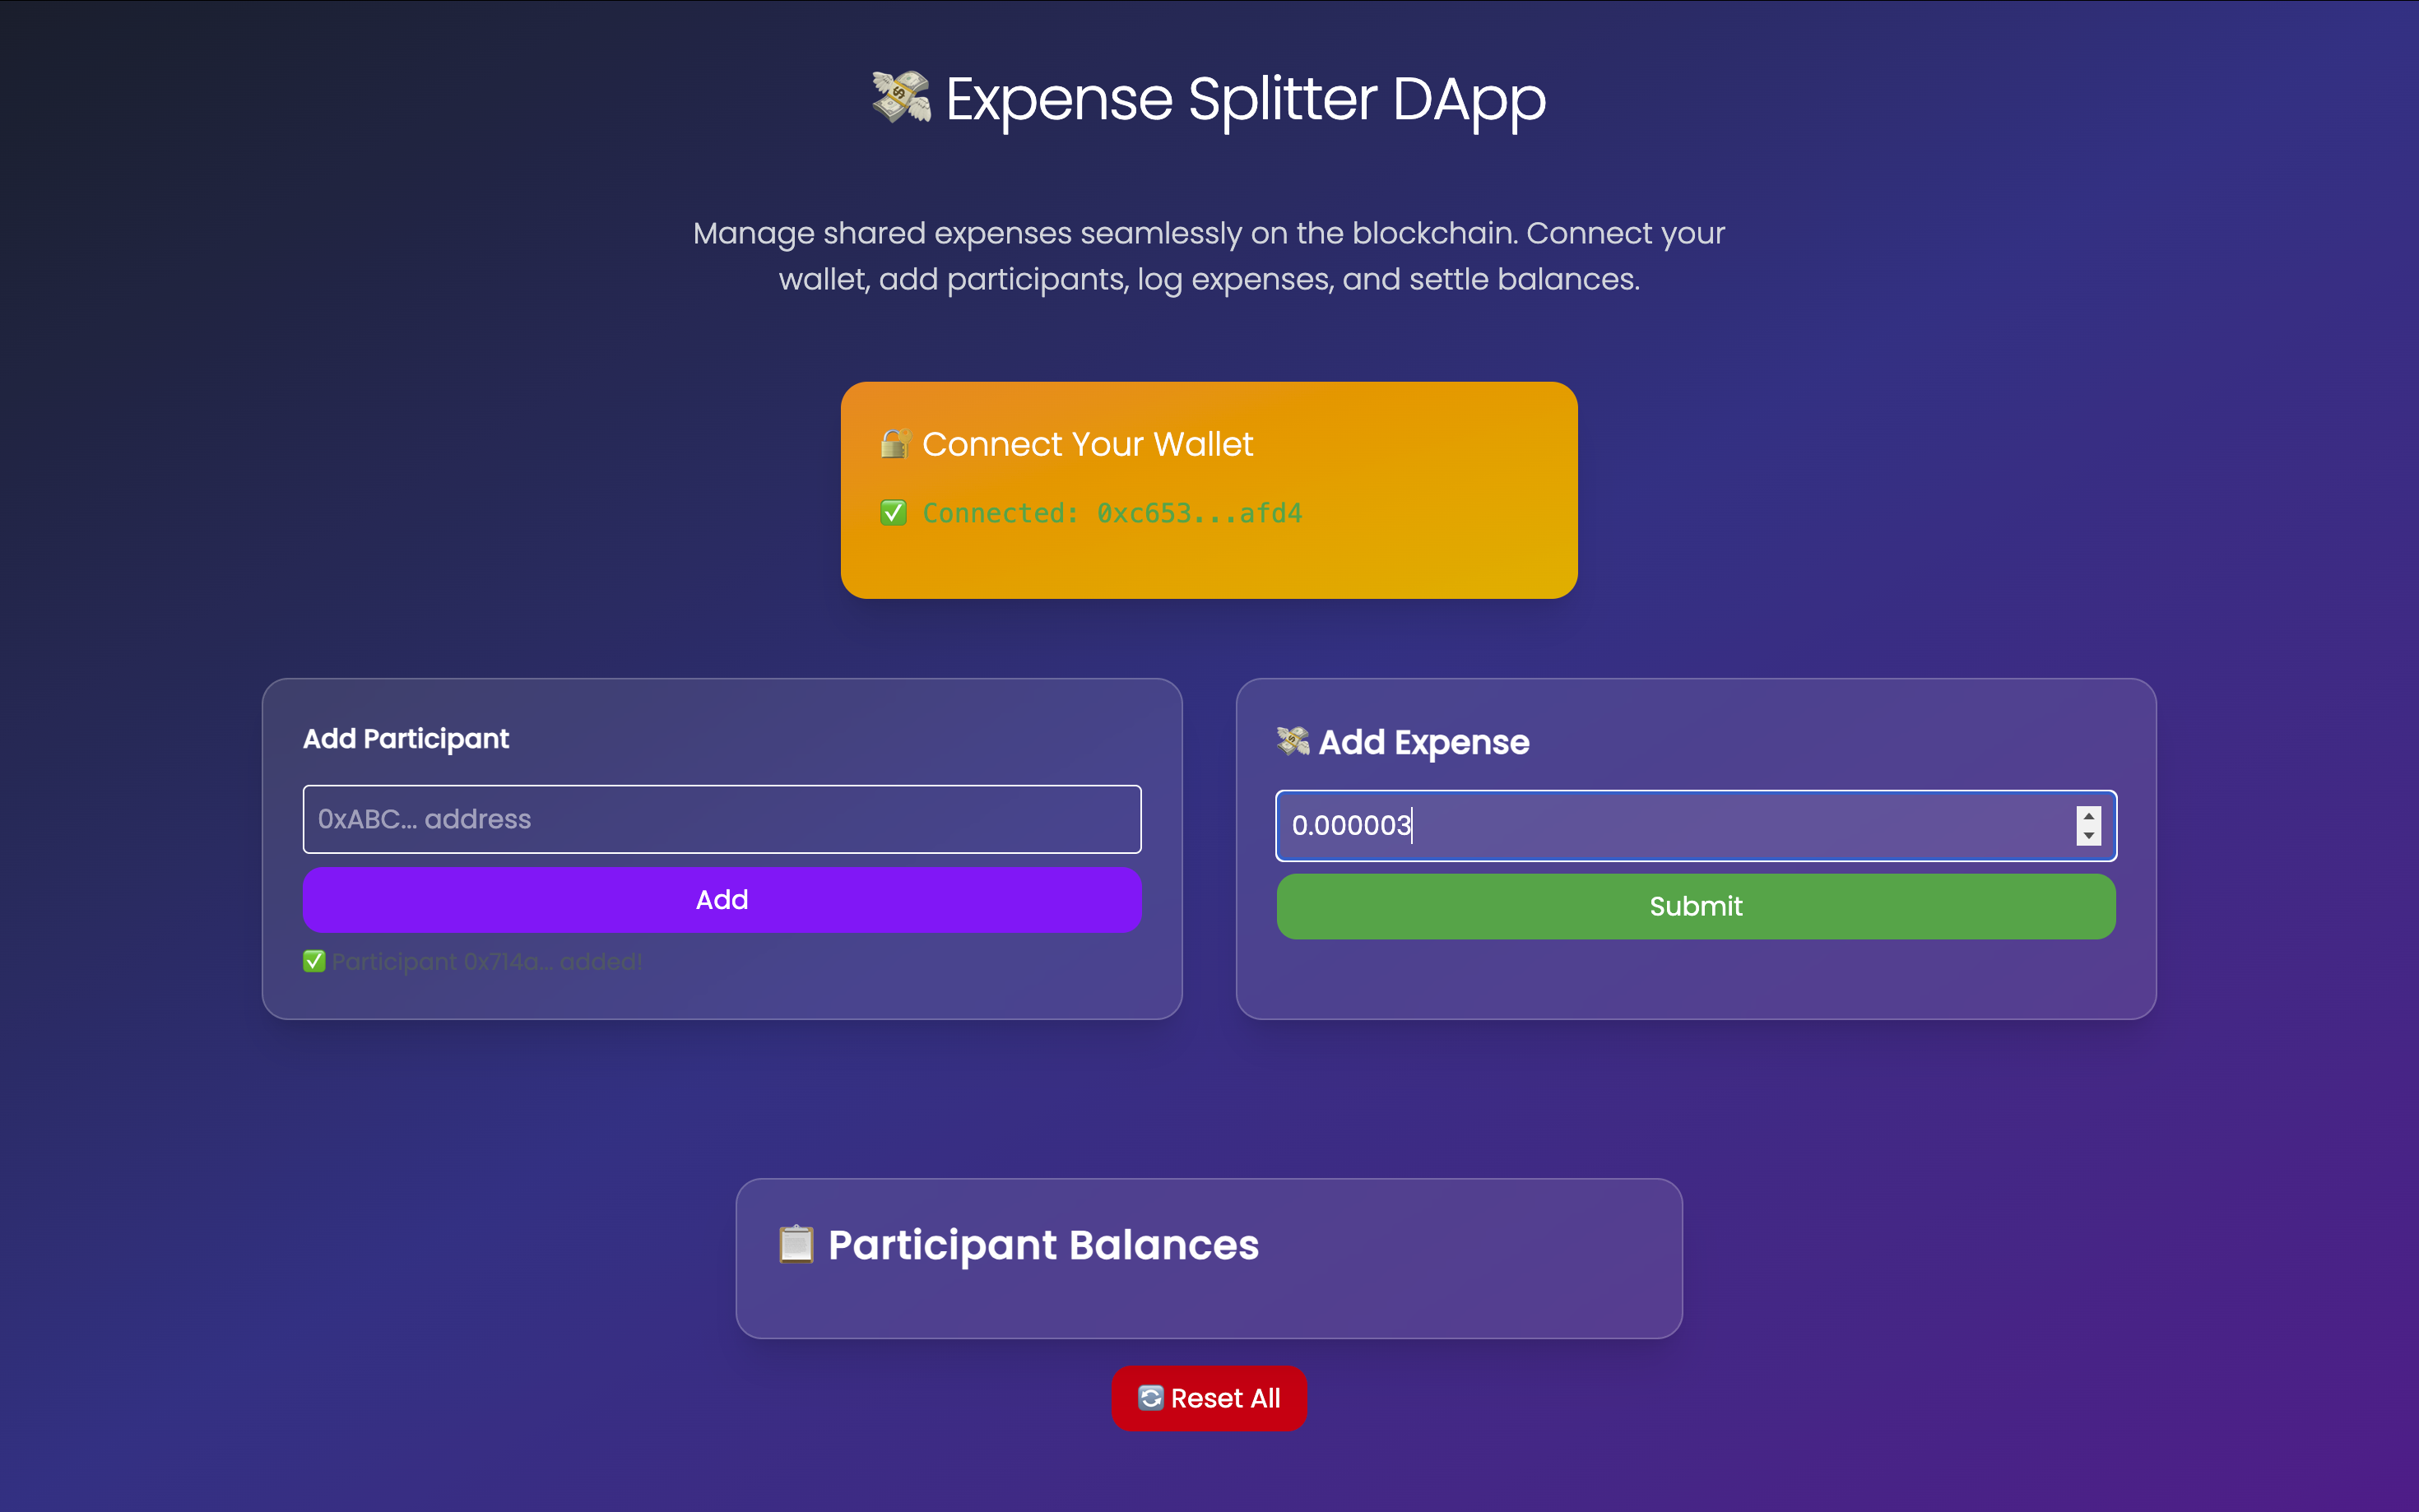
\includegraphics[width=0.7\textwidth]{add_expense.png}
    \caption{Add expenses to Decentralized Expense Splitter DApp.}
    \label{fig:add_expense}
\end{figure}
\begin{figure}[h]
    \centering
    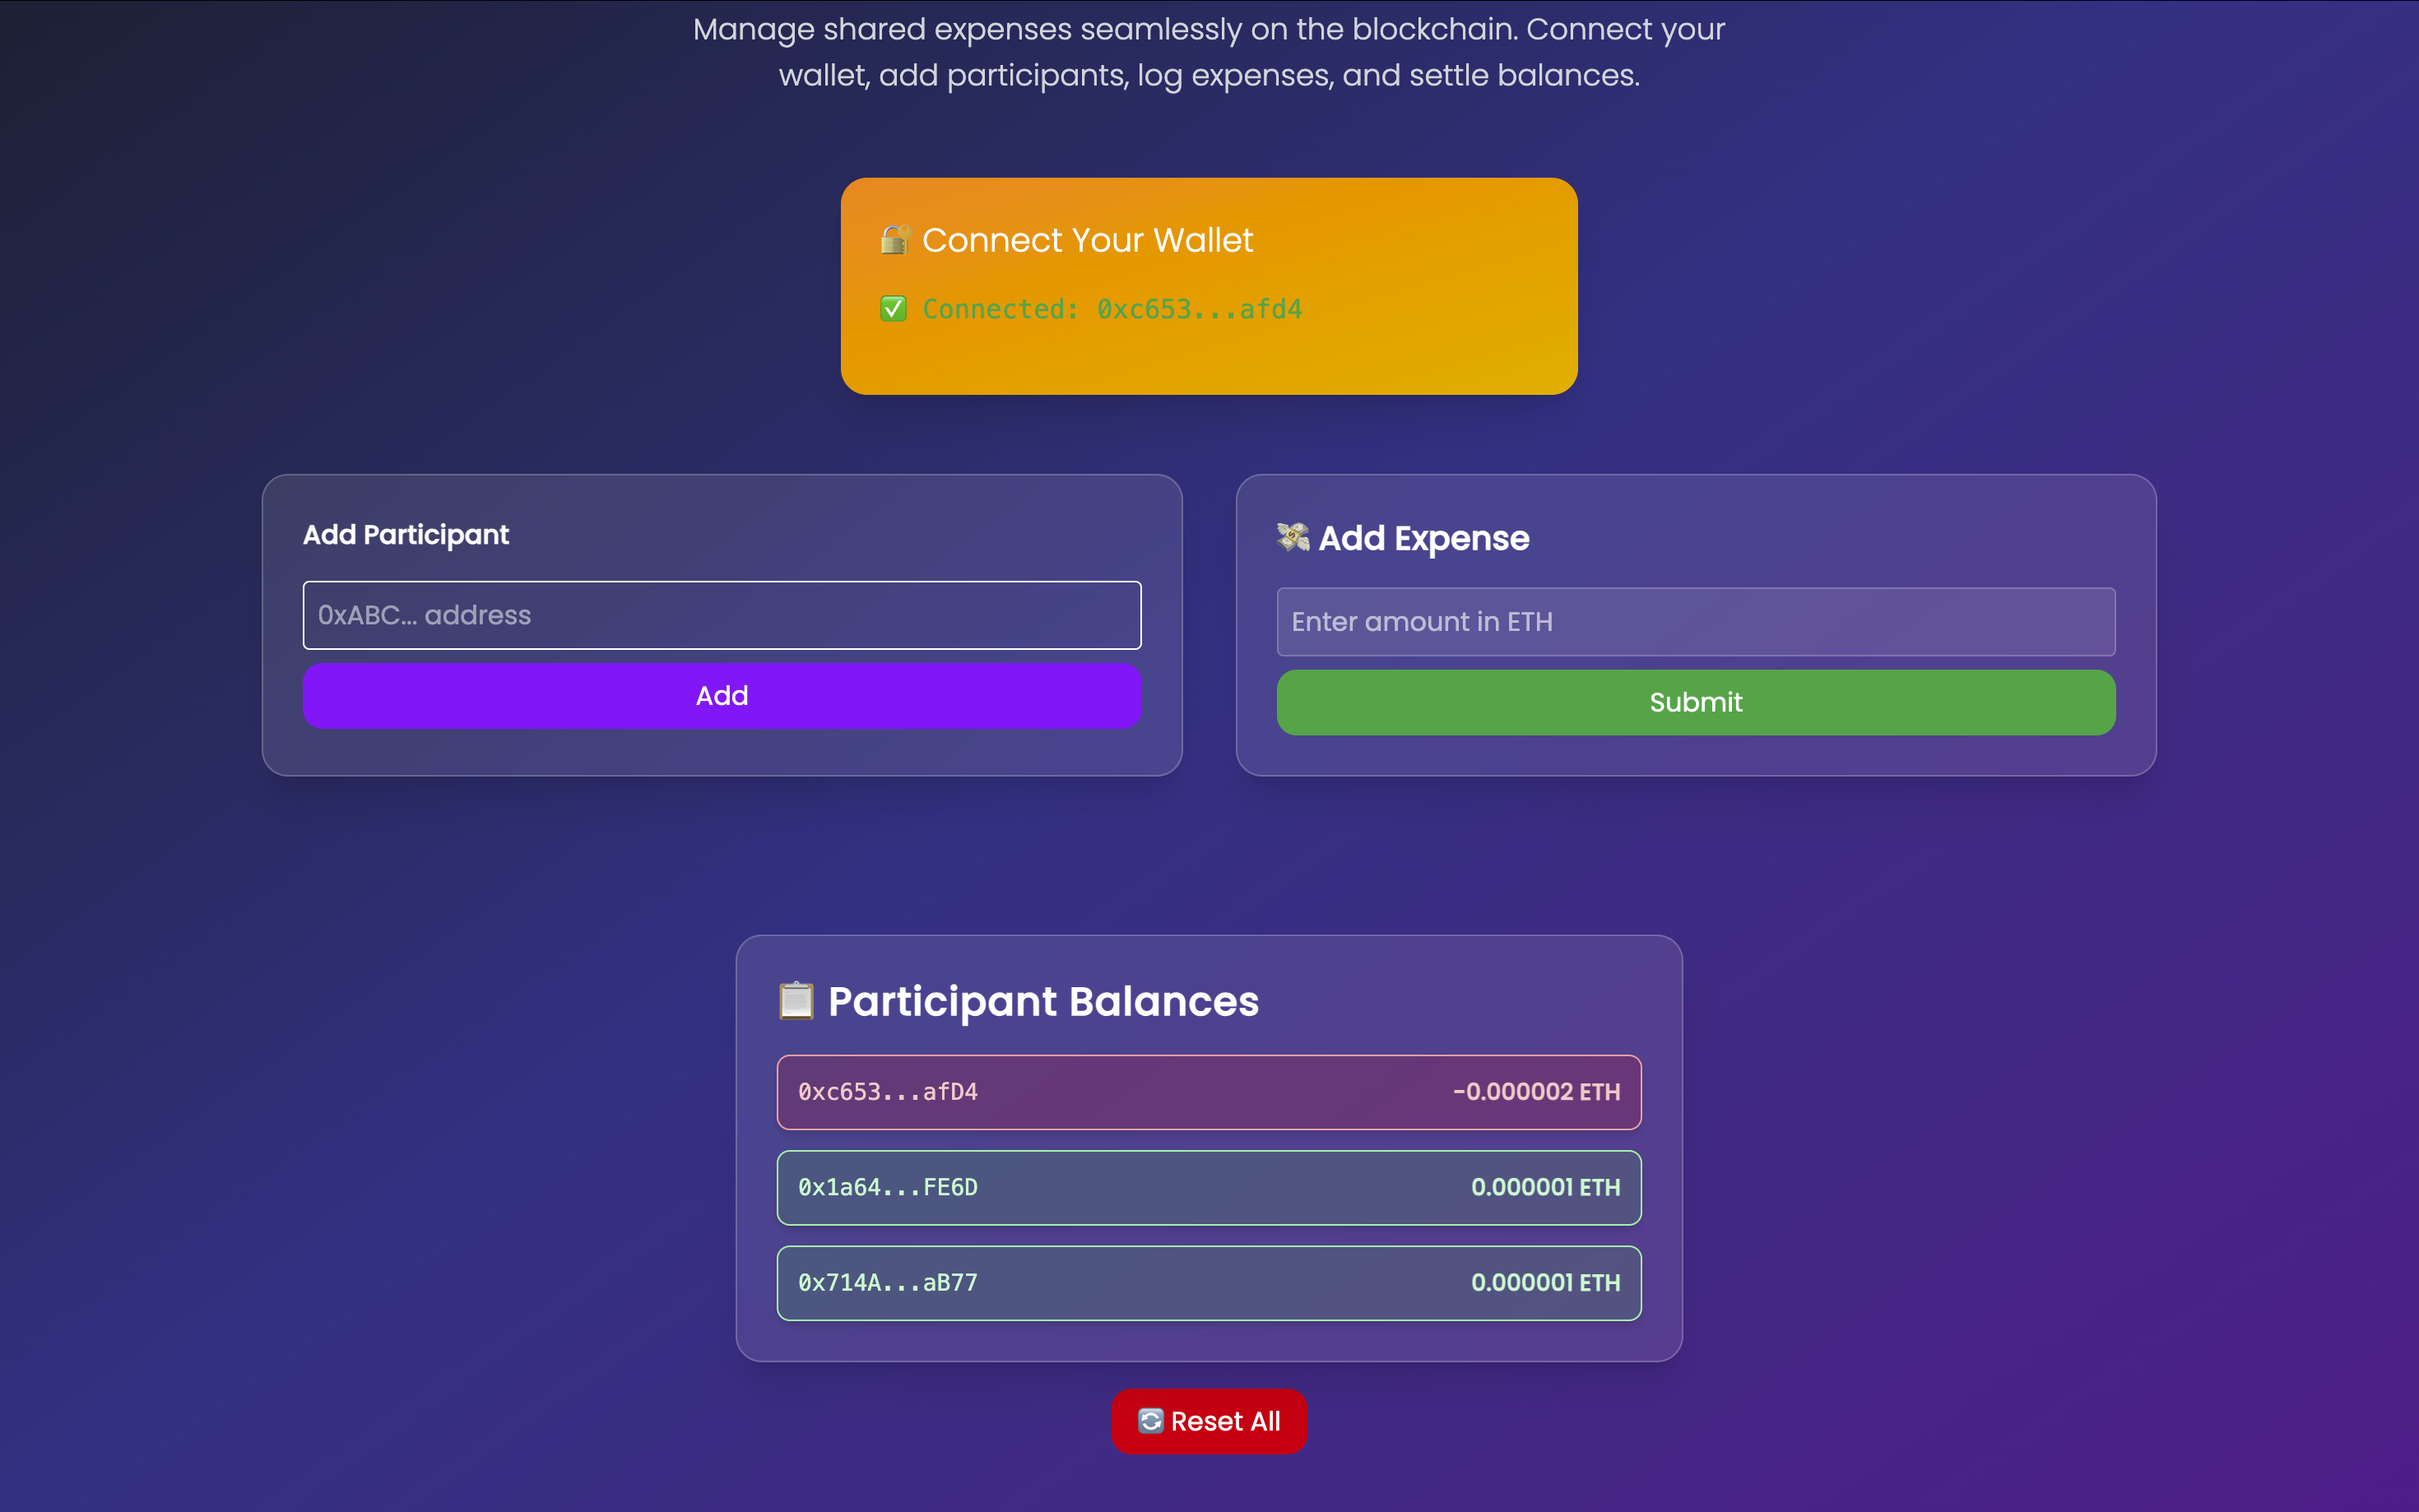
\includegraphics[width=0.7\textwidth]{balance_list.png}
    \caption{View balances in Decentralized Expense Splitter DApp.}
    \label{fig:balance_list}
\end{figure}
\begin{figure}[h]
    \centering
    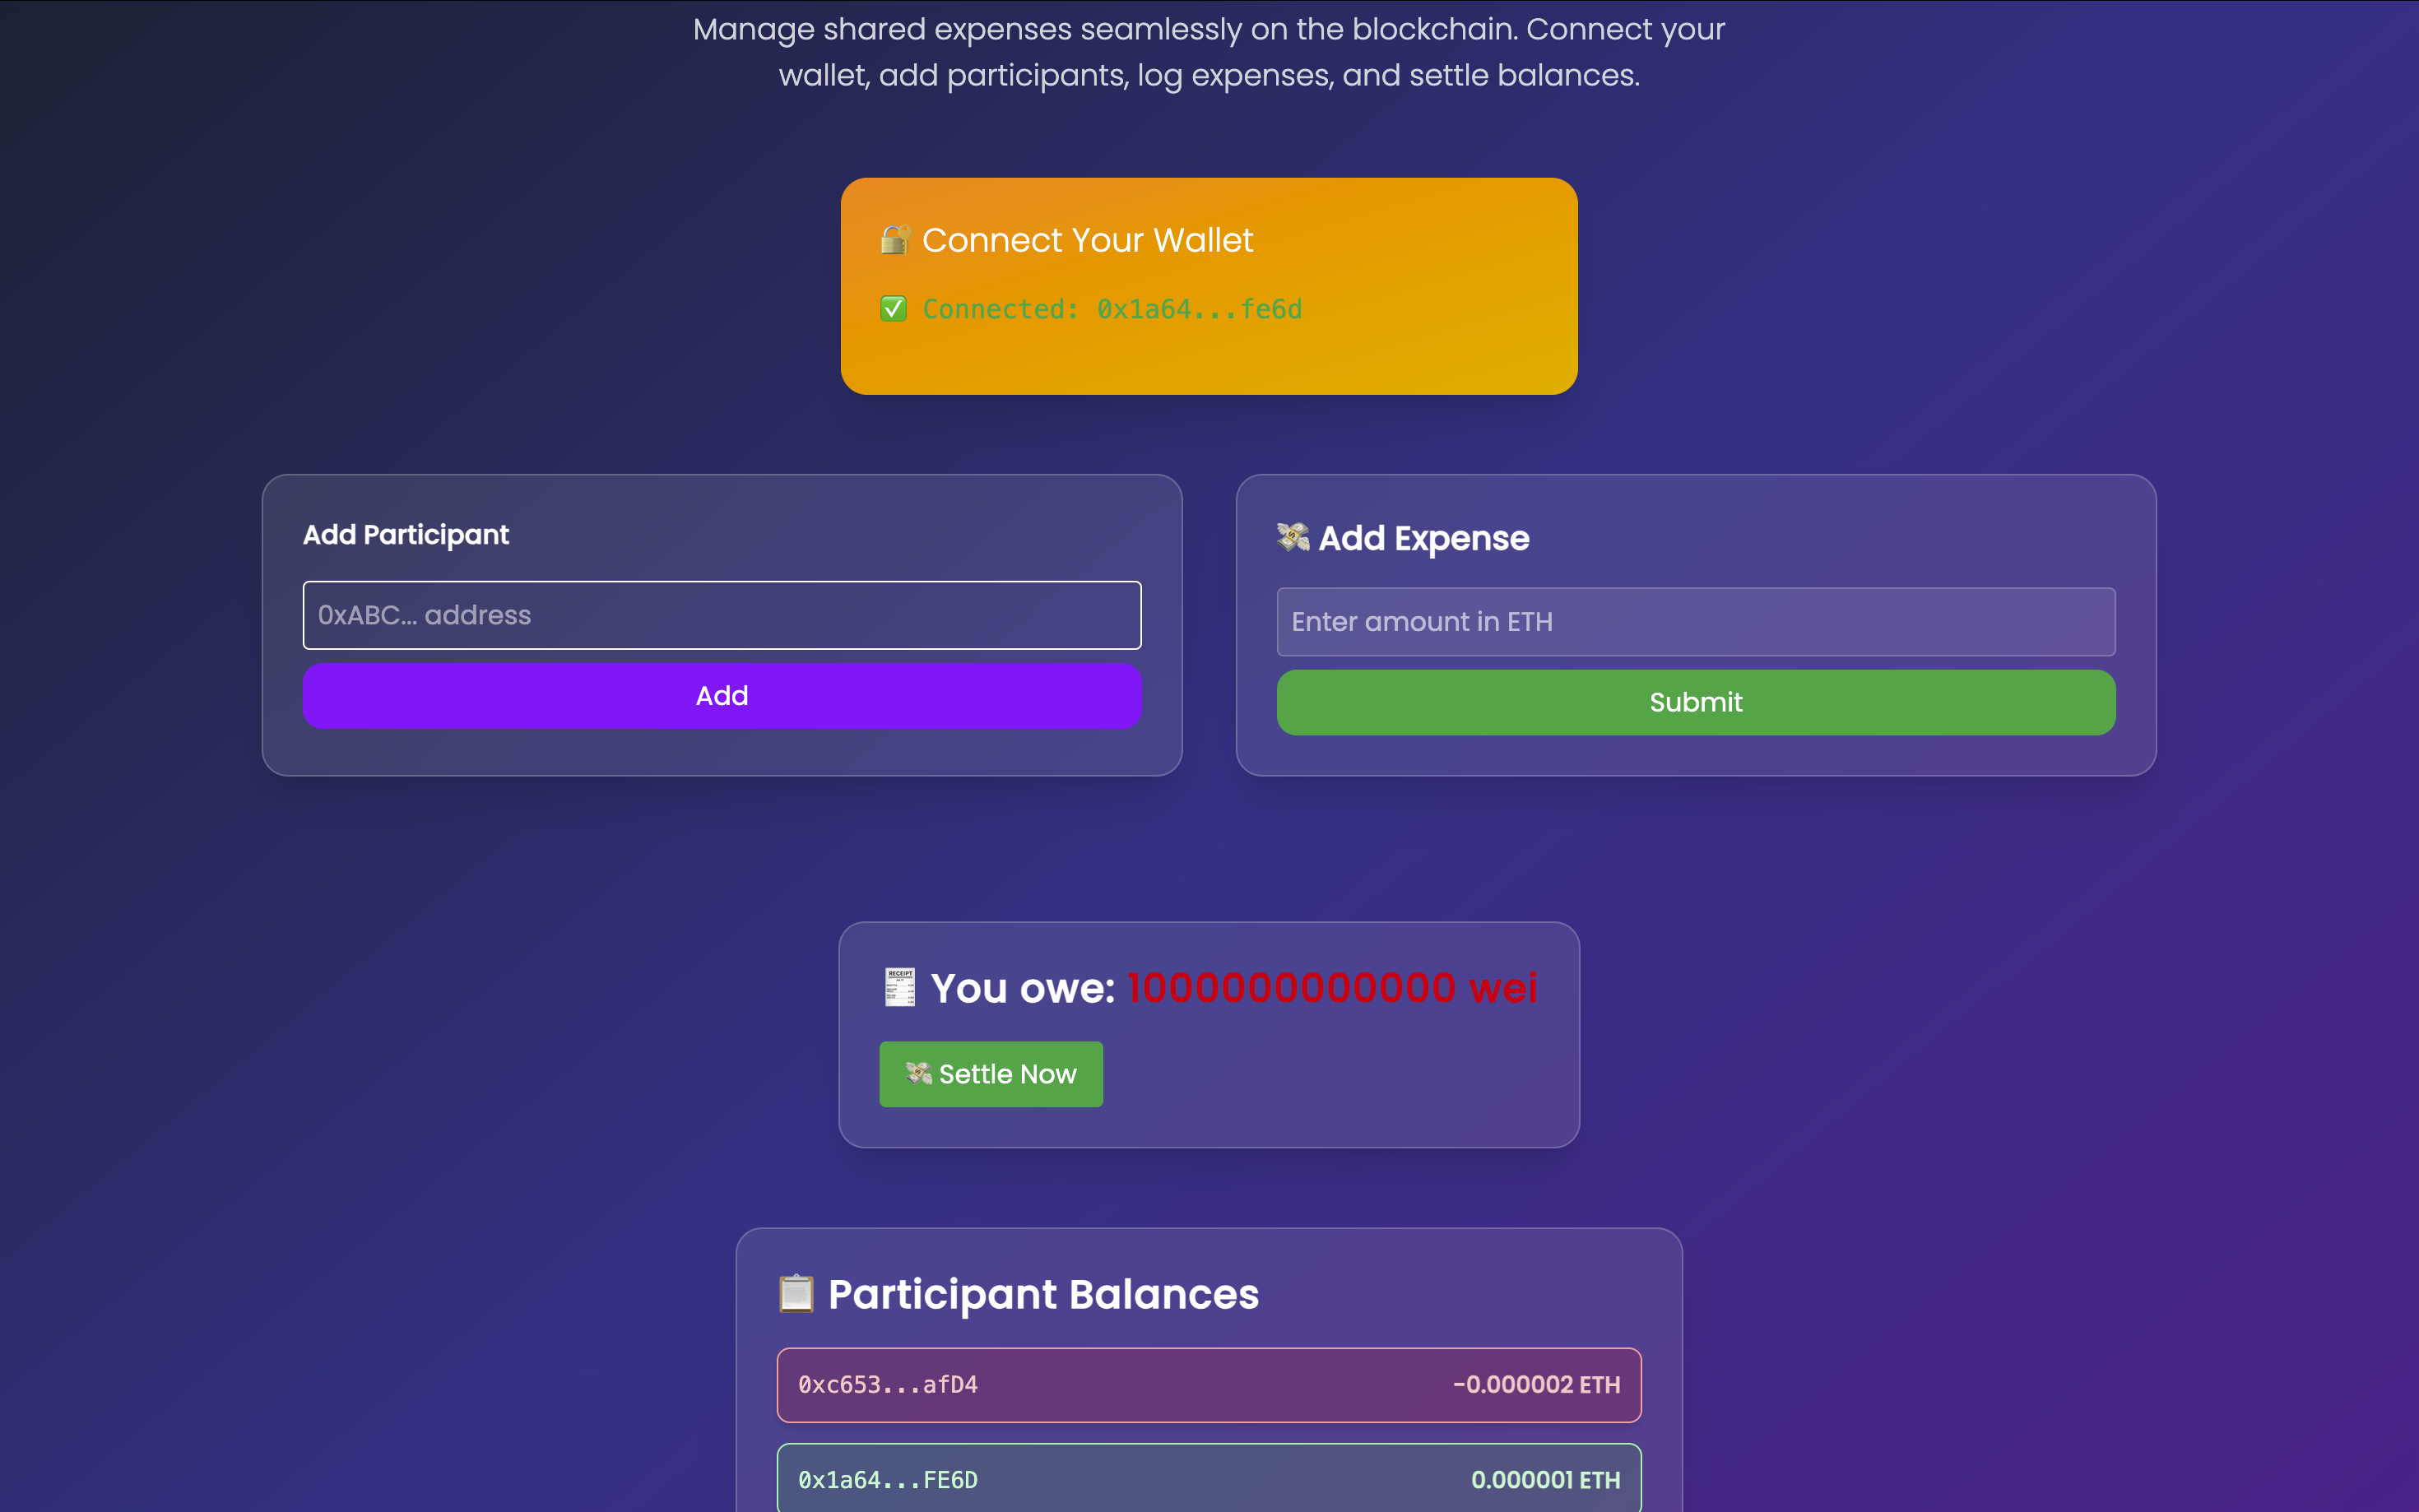
\includegraphics[width=0.7\textwidth]{settle.png}
    \caption{Settle debts in Decentralized Expense Splitter DApp.}
    \label{fig:settle}
\end{figure}
\section{Project Demo and Source Code}

You can try the Expense Splitter DApp live or view the source code:

\begin{itemize}
    \item \textbf{Live Demo:} \href{https://expense-splitter-akn7qyy37-hari-hara-tejas-projects.vercel.app/}{https://expense-splitter-akn7qyy37-hari-hara-tejas-projects.vercel.app/}
    \item \textbf{GitHub Repository:} \url{https://github.com/hariharateja/Expense_splitter_blockchain}
\end{itemize}
\textbf{Why Expense Splitter?}
We friends often go out together, and managing shared expenses can be a hassle. The Expense Splitter DApp simplifies this process by automating expense tracking and settlement, ensuring transparency and fairness among participants. It eliminates the need for manual calculations and reduces the chances of disputes over who owes what.
\newline
\textbf{Technologies Used:}
\begin{itemize}
    \item Solidity for smart contract development
    \item React for frontend development
    \item web3.js for blockchain interaction
    \item Tailwind CSS for styling
    \item Ethers.js for wallet integration
    \item Framer Motion for animations
    \item Vercel for deployment
\end{itemize}
\textbf{Conclusion:}
The Expense Splitter DApp is a practical example of how blockchain technology can enhance everyday activities like expense management. By leveraging smart contracts, we can create decentralized applications that are secure, transparent, and efficient. This project showcases the potential of blockchain in simplifying group activities and fostering trust among participants.
\section{Challenges faced}
\begin{itemize}
    \item \textbf{Understanding Solidity Syntax:} Initially, the syntax and structure of Solidity were challenging. However, with practice and reference to documentation, I became more comfortable with it.
    \item \textbf{Gas Optimization:} Ensuring that the smart contract was gas-efficient was a significant challenge. I had to learn about various optimization techniques, such as using smaller data types and minimizing storage operations.
    \item \textbf{Debugging Smart Contracts:} Debugging smart contracts can be tricky due to the immutable nature of blockchain. I had to rely on tools like Remix and Hardhat for testing and debugging, which helped identify issues before deployment.
    \item \textbf{Frontend Integration:} Integrating the smart contract with the frontend using web3.js and React posed challenges, especially with handling asynchronous calls and managing state. I had to ensure that the frontend correctly reflected the contract's state and handled user interactions smoothly.
    \item \textbf{Wallet Integration:} Setting up wallet connections (like MetaMask) and ensuring secure transactions was another hurdle. I had to understand how to handle user accounts, sign transactions, and manage errors related to wallet interactions.
    \item \textbf{Testing on Testnets:} Deploying the contract on testnets (like Ropsten or Rinkeby) required understanding how to obtain test Ether and manage different network configurations. I faced issues with network connectivity and had to troubleshoot them to ensure successful deployments.
    \item \textbf{User Experience Design:} Designing a user-friendly interface that effectively communicates with the smart contract was a challenge. I had to consider how users would interact with the DApp, ensuring that it was intuitive and provided clear feedback on actions like adding expenses or settling debts.
    \item \textbf{Security Considerations:} Ensuring the smart contract was secure against common vulnerabilities (like reentrancy attacks or integer overflows) was crucial. I had to learn about best practices in smart contract security and implement them in my code.
    \item \textbf{Deployment Issues:} Deploying the contract to the Ethereum mainnet required careful consideration of gas prices and transaction fees. I had to monitor the network conditions and adjust my deployment strategy accordingly to avoid high costs.
\end{itemize}
These challenges provided valuable learning experiences and helped me gain a deeper understanding of blockchain development, smart contracts, and decentralized applications. Overcoming these obstacles has made me more confident in my ability to build and deploy smart contracts and develop DApps.
\section{Quantum Proofing}
\subsection{Introduction}
So Blockchain is built on the fundamental concept of cryptography for the private public key matters. Once Quantum Computers are fully developed then just like many other traditional cryptography methods, this will fail too. So we need to see what can be done about it. I would talk mainly about quantum-proofing cryptography not blockchain specifically since it would be too narrow downed.
\subsection{Basic Cryptography}
Cryptographic algorithms like RSA (one of the most famous one) and some others rely on multiplying 2 very large prime numbers to get a very very large number (duh). So very similar to how private and public key worked earlier (I am lazy to use references in L A T EX). I will not get into details of the RSA algorithm and well its complicated, but it is heavily relient on the fact that it is difficult to extract the 2 prime numbers from the very very large number (Source: trust me bro) So normal computers take a lot of time for this, but quantum computers wont (Source: Just trust me bro). Because computers work on bits that is 0s and 1s (binary again duh) but quantum computers qubits which can be present in a superposition of 0s and 1s.
\subsection{Shors Algorithm}
Shor’s algorithm, launched in 1994 by mathematician Peter Shor, is a quantum algorithm specialized in efficiently factorizing large numbers, a challenge for traditional computers. As i said, factorizing the very very large number is important which is made faster by this.
\subsection{Grover’s Algorithm}
Grover's algorithm, developed by Lov Grover in 1996, is a quantum algorithm that provides a quadratic speedup for unstructured search problems. While it doesn't directly address the factorization problem like Shor's algorithm, it has implications for searching through large databases or solving certain NP-complete problems more efficiently than classical algorithms.
\subsection{Lattice-Based Cryptography}
Doing this separately because i really liked it. Soo how does this work? Imagine you have 2 vectors in R2 , say (1,0) and (0,1). Now any integer linear combination of these 2 vectors is the lattice of these 2 vectors. Now lets say i want you to find the closest lattice point from (5.1,7.9). well u know the answer is (5,8) do this easily because you have a set of ”good” vectors. but lets say i give you something close to parallel like, (10000019,10000079) and (10000057,10000103). Its going to be difficult to find the closest lattice point to that. so i have the vectors 1,0 and 0,1 but i share my lattice using the
vectors (10000019,10000079) and (10000057,10000103). The problem comes with saying
for sure that a certain lattice point is closest to it. Now imagine this to be in 1000
dimensions instead of 2.
\newline
So now if i have to send a message to Nirav, Nirav will have made his lattice using (1,0) and (0,1) which he will keep to himself. he will share the basis (10000019,10000079) and (10000057,10000103) to everyone. Now for example my message is (89,21). So my lattice point is 89*(10000019,10000079) + 21*(10000057,10000103). and then i will add a little noise to it. now for anyone without (1,0) and (0,1) it will be difficult to find the lattice point closest to the noised point since you wont be able to say for sure if its the closest since going closer in 1 dimension might make you so much farther in the other 999. I know i havent taken the best examples but you get my point. This is called the GGH algorithm which even though isn’t very safe it is still hopeful for what lattice based crytographic techniques we have in the future.
\subsection{Conclusion}
Quantum-proofing cryptography is an essential step in ensuring the security and integrity of blockchain systems in the face of advancing quantum computing technology. By adopting quantum-resistant algorithms, such as lattice-based cryptography, hash-based signatures, and multivariate polynomial cryptography, we can mitigate the risks posed by quantum attacks. It is crucial for developers, researchers, and organizations to stay informed about the latest advancements in quantum-proofing techniques and to implement them proactively in their blockchain applications. As quantum computing continues to evolve, ongoing research and collaboration within the blockchain community will be vital to maintaining the security and trustworthiness of decentralized systems.
\section{Project Conclusion}
In this report, we have explored the fundamentals of blockchain technology, focusing on Ethereum and smart contracts. We discussed the architecture of Ethereum, the role of smart contracts, and how they can be deployed and interacted with using tools like Remix IDE and MetaMask. We also covered best practices for writing efficient and secure smart contracts, including gas optimization techniques and the importance of testing and verification.
Furthermore, we provided a practical example of a smart contract and demonstrated how to connect it with a frontend application using web3.js or ethers.js. The report also highlighted the challenges faced during the development process and the importance of quantum-proofing cryptography in the context of blockchain security.
\newline
Overall, this report serves as a comprehensive guide for understanding and working with blockchain technology, particularly in the context of Ethereum and smart contracts. It provides a solid foundation for further exploration and development in the field of decentralized applications and blockchain solutions.
\section{signing off}
In conclusion, the rapid advancement of blockchain technology and its potential applications necessitate a proactive approach to security and scalability. By addressing the challenges and exploring innovative solutions, we can pave the way for a more secure and efficient decentralized future.
\newline
This report has provided a comprehensive overview of blockchain fundamentals, smart contract development, and the integration of frontend applications. It has also highlighted the importance of quantum-proofing cryptography to ensure the long-term security of blockchain systems. As we continue to explore the possibilities of blockchain technology, it is crucial to stay informed about the latest developments and best practices in the field.
\newline
We hope this report serves as a valuable resource for developers, researchers, and enthusiasts interested in blockchain technology. By understanding the principles and practices outlined in this report, individuals can contribute to the ongoing evolution of blockchain and help shape the future of decentralized applications.
\newline
\textbf{Thank you SOS! and My Mentor: Yuvraj Gupta for your guidance and support throughout this project. Your insights and expertise have been invaluable in shaping my understanding of blockchain technology and smart contract development. I look forward to applying the knowledge gained from this project in future endeavors and contributing to the exciting field of blockchain innovation.}
\section{References}
\begin{itemize}
    \item Ethereum Documentation: \url{https://docs.ethereum.org/}
    \item Solidity Documentation: \url{https://docs.soliditylang.org/}
    \item Remix IDE: \url{https://remix.ethereum.org/}
    \item MetaMask: \url{https://metamask.io/}
    \item Web3.js Documentation: \url{https://web3js.readthedocs.io/}
    \item Ethers.js Documentation: \url{https://docs.ethers.io/}
    \item Solidity Gas Optimization Techniques: \url{https://docs.soliditylang.org/en/latest/internals/layout_in_storage.html}
    \item Quantum Proofing Cryptography: \url{https://en.wikipedia.org/wiki/Quantum-resistant_cryptography}
    \item Shor's Algorithm: \url{https://en.wikipedia.org/wiki/Shor%27s_algorithm}
    \item Grover's Algorithm: \url{https://en.wikipedia.org/wiki/Grover's_algorithm}
    \item Lattice-Based Cryptography: \url{https://en.wikipedia.org/wiki/Lattice-based_cryptography}
    \item Expense Splitter DApp Source Code: \url{https://github.com/hariharateja/Expense_splitter_blockchain}
\end{itemize} 
\end{document}
